%!TEX root = ../main.tex
\chapter{Risoluzione di Equazioni Differenziali Ordinarie}
\label{chap:edo}

In questo capitolo ci dedicheremo alle EDO, \textbf{equazioni differenziali ordinarie}\index{equazioni differenziali ordinarie}, ovvero equazioni dalla forma generale:
\begin{equation*}
	F\left(x,y,y',y'',\cdots,y^{(n)} \right) = 0,
\end{equation*}
dove quindi sono coinvolte le derivate di $y$, la funzione incognita da determinare, ed eventualmente la variabile $x$, cioè l'argomento della $y$.

Queste equazioni sono importantissime, perché consentono di descrivere in modo molto accurato tantissimi fenomeni fisici, anche se in realtà questi si descrivono più propriamente con le EDP, \textbf{equazioni alle derivate parziali}\index{equazioni alle derivate parziali}.
Nelle EDP non c'è dipendenza da una sola variabile, ma da più variabili, quindi naturalmente si potrà derivare la funzione incognita rispetto a ciascuna delle variabili, eventualmente più volte.
Tipicamente quando la dipendenza è da una sola variabile essa si può interpretare come un tempo o uno spazio. Quando però si vuole studiare l'evoluzione nel tempo di un sistema in 3D è chiaro che servono $3+1$ variabili, quindi una EDP.
Un aspetto interessante è che a volte la risoluzione delle EDP può essere ridotta a una EDO, per cui anche lo studio che affronteremo adesso sarà fondamentale per la modellistica fisica e le simulazioni numeriche.

\textit{Esempio.}
Supponiamo di avere una popolazione di batteri in un ambiente limitato nel quale non possono convivere più di $B$ batteri contemporaneamente. Supponiamo inoltre che all'istante in cui inizia l'esperimento, il numero di batteri sia $y_{0} \ll B$ e che il fattore di crescita dei batteri sia pari a una costante $r >0$. Come cambia nel tempo il numero di batteri?

Per scrivere un modello matematico di questo problema, dobbiamo anzitutto definire la quantità di interesse: sia $y(t)$ il numero di batteri all'istante $t$.

I dati sono:
\begin{itemize}
\item $y(0) =y_{0}$, la quantità di batteri all'istante iniziale $t=0$;
\item $r$, il fattore di crescita;
\item $B$, il numero massimo di batteri che possono coesistere.
\end{itemize}
Supponiamo $y \in C^{1} $: se a un certo punto $y(t) =B$, la derivata di $y(t)$ si deve annullare in quel punto.

Scriviamo ora il modello:
\begin{equation*}
\begin{cases}
\frac{\dy(t)}{\dt} =r\ y(t)\left( 1-\frac{y(t)}{B}\right)\\
y(0) =y_{0}.
\end{cases}
\end{equation*}
Esso è un esempio di \textbf{equazione funzionale}\index{equazione!funzionale}, in quanto i suoi elementi, inclusa l'incognita $y(t)$, sono funzioni e non quantità algebriche.
In particolare, è un'\textit{equazione differenziale ordinaria} (EDO), poiché presenta operazioni di derivazione.
\textit{Ordinaria} significa che non presenta derivate parziali.
L'\textit{ordine} di tale equazione è invece il più alto grado di derivazione presente.
In particolare, ci concentreremo sulle equazioni differenziali di primo ordine.

Supponiamo ora di avere due popolazioni di batteri distinte e in competizione tra loro. Indichiamo con $y_{1}(t)$ e $y_{2}(t)$ il numero di batteri rispettivamente della prima e della seconda popolazione. In questo caso il modello matematico diventa:
\begin{equation*}
\begin{cases}
\frac{\dy_{1}}{\dt} =r_{1} y_{1}( 1-b_{1} y_{1} -d_{2} y_{2})\\
\frac{\dy_{2}}{\dt} =r_{2} y_{2}( 1-b_{2} y_{2} -d_{1} y_{1})\\
y_{1}(0) =y^{0}_{1}\\
y_{2}(0) =y^{0}_{2}
\end{cases}
\end{equation*}
dove
\begin{itemize}
\item $r_{1} ,r_{2}$ sono i fattori di crescita delle due popolazioni
\item $b_{1} ,b_{2}$ sono fattori legati alla disponibilità di nutrienti, e quindi alla sopravvivenza delle singole popolazioni
\item $d_{1} ,d_{2}$ sono fattori che governano le interazioni, cioè la competizione, tra le due popolazioni.
\end{itemize}

La soluzione è della forma
\begin{equation*}
\y(t) =\begin{pmatrix}
y_{1}(t)\\
y_{2}(t)
\end{pmatrix}.
\end{equation*}

% \textit{[Lezione 17 (28-04-2020)]}
\section{Problema di Cauchy}
In generale, il problema matematico modello che vogliamo studiare si può così formulare:
Sia $I=[ t_{0} ,t_{0} +T]$ e $f:I\times \mathbb{R}\rightarrow \mathbb{R}$, vogliamo trovare $y(t) :I\rightarrow \mathbb{R}$ tale che
\begin{equation}
\tag{PC}
\begin{cases}
y'(t) =f( t,y(t))\\
y( t_{0}) =y_{0}
\end{cases} \quad t\in I
\label{eq:problema-di-cauchy}
\end{equation}
dove $y_{0} \in \mathbb{R}$ è assegnato.

\textit{Osservazione.}
Se la funzione $f$ è continua rispetto a $t$, possiamo integrare la prima equazione di \eqref{eq:problema-di-cauchy} tra $t_{0}$ e $t$ ottenendo la seguente formulazione:
\begin{equation*}
y(t) =y_{0} +\int\nolimits ^{t}_{t_{0}} f( \tau ,y( \tau )) \de\tau.
\end{equation*}
Ci interessa conoscere:
\begin{enumerate}
\item se \eqref{eq:problema-di-cauchy} ammette una sola soluzione;
\item la regolarità di questa soluzione;
\item se la soluzione sia stabile rispetto ai dati, ovvero se dipenda con continuità da essi.
\end{enumerate}

\begin{definition}
[Funzione lipschitziana]
\index{funzione!lipschitziana}
Una funzione $g:I\rightarrow \mathbb{R}$ è detta lipschitziana se esiste una costante $L$ tale che
\begin{equation*}
| g( x) -g( y)| \leqslant L| x-y| ,\ \ \forall x,y\in I.
\end{equation*}
Inoltre la costante migliore, cioè la più bassa possibile che rispetti la disuguaglianza, viene detta costante di Lipschitz.
\end{definition}

\begin{theorem}
[Esistenza della soluzione del \eqref{eq:problema-di-cauchy}]
\index{teorema!della soluzione del problema di cauchy}
Supponiamo che la funzione $f( \cdot ,\cdot )$ sia continua rispetto a entrambe le variabili, e che sia lipschitziana rispetto al secondo argomento.
Allora la soluzione del Problema di Cauchy \eqref{eq:problema-di-cauchy} esiste ed è unica, e inoltre $y\in C^{1}(I)$.
\label{thm:esistenza-unicita-PC}
\end{theorem}

Il teorema risponde ai primi due punti. Al fine di studiare il terzo punto, ovvero la stabilità di \eqref{eq:problema-di-cauchy}, consideriamo il seguente problema perturbato:
\begin{equation*}
(\widetilde{\text{PC}}) \ \begin{cases}
z'(t) =f( t,z(t)) +\delta (t)\\
z(0) =y_{0} +\delta _{0}
\end{cases} \quad t\in I
\end{equation*}
dove $\delta _{0} \in \mathbb{R}$ e $\delta (t)$ è una funzione continua in $I$. Vogliamo caratterizzare la sensibilità di $z(t)$ alle perturbazioni $\delta _{0}$ e $\delta (t)$. Questo è il concetto di stabilità secondo Lyapunov.

\begin{definition}
[Stabilità secondo Lyapunov]
\index{stabilità!secondo Lyapunov}
Sia $I=[ t_{0} ,t_{0} +T]$ un intervallo limitato $( T< +\infty )$.
Diciamo che \eqref{eq:problema-di-cauchy} è stabile secondo Lyapunov se per ogni perturbazione $( \delta _{0} ,\delta (t))$ tale che
\begin{equation*}
| \delta _{0}| < \varepsilon ,\quad | \delta (t)| < \varepsilon ,\quad \forall t\in I,\quad \varepsilon  >0,
\end{equation*}
con $\varepsilon $ sufficientemente piccolo da garantire che $(\widetilde{\text{PC}})$ ammetta una e una sola soluzione, allora esiste $c >0$, indipendente da $\varepsilon $, tale che
\begin{equation}
| y(t) -z(t)| < c\ \varepsilon ,\quad \forall t\in I.
\label{eq:stabilita-lyapunov}
\end{equation}
\end{definition}

\begin{definition}
[Stabilità asintotica]
\index{stabilità!asintotica}
Sia $I$ un intervallo superiormente illimitato.
Si dice che \eqref{eq:problema-di-cauchy} è asintoticamente stabile se vale \eqref{eq:stabilita-lyapunov} e inoltre
\begin{equation*}
\lim _{t\rightarrow \infty }| y(t) -z(t)| =0
\end{equation*}
purché $| \delta (t)| \rightarrow 0$ per $t\rightarrow \infty $.
\end{definition}

Enunciamo ora un lemma utile nella dimostrazione di risultati di stabilità.
\begin{lemma}
[Gronwall]
\index{lemma!di Gronwall}
Sia $p$ una funzione integrabile e non negativa sull'intervallo $[ t_{0} ,t_{0} +T]$ e siano $g$ e $\varphi $ due funzioni continue su $[ t_{0} ,t_{0} +T]$, con $g$ non decrescente. Allora
\begin{equation*}
\varphi (t) \leqslant g(t) +\int\nolimits ^{t}_{t_{0}} p(s) \varphi (s) \ds \ \ \Rightarrow \ \ \varphi (t) \leqslant g(t)\exp\left(\int\nolimits ^{t}_{t_{0}} p(s) \ds\right).
\end{equation*}
\end{lemma}

\begin{theorem}
[Stabilità]
\index{teorema!della stabilita}
Sia $f( \cdot ,\cdot )$ lipschitziana rispetto al secondo argomento. Allora \eqref{eq:problema-di-cauchy} è asintoticamente stabile.
\label{thm:stabilita-PC}
\end{theorem}

\textit{Dimostrazione.}
Sia $y(t)$ la soluzione di \eqref{eq:problema-di-cauchy} e sia $z(t)$ la soluzione di $(\widetilde{\text{PC}})$. Definiamo $w(t) =z(t) -y(t)$. Si ha, con $t\in I$:
\begin{equation*}
\begin{cases}
w'(t) =f( t,z(t)) +\delta (t) -f( t,y(t))\\
w( t_{0}) =\cancel{y_{0}} +\delta _{0} -\cancel{y_{0}}.
\end{cases}
\end{equation*}
Integriamo entrambi i membri della prima equazione tra $t_{0}$ e $t$:
\begin{align*}
\int\nolimits ^{t}_{t_{0}} w'(s) \ds & =\int\nolimits ^{t}_{t_{0}}[ f( s,z(s)) +\delta (s) -f( s,y(s))] \ds\\
w(t) -w( t_{0}) & =\int\nolimits ^{t}_{t_{0}}[ f( s,z(s)) -f( s,y(s))] \ds+\int\nolimits ^{t}_{t_{0}} \delta (s) \ds\\
w(t) & =\delta _{0} +\int\nolimits ^{t}_{t_{0}}[ f( s,z(s)) -f( s,y(s))] \ds+\int\nolimits ^{t}_{t_{0}} \delta (s) \ds
\end{align*}
Passiamo al modulo e otteniamo:
\begin{equation*}
| w(t)| \leqslant | \delta _{0}| +\int\nolimits ^{t}_{t_{0}}| f( s,z(s)) -f( s,y(s))| \ds+\int\nolimits ^{t}_{t_{0}}| \delta (s)| \ds.
\end{equation*}
Ricordando che $f$ è lipschitziana per ipotesi:
\begin{equation*}
| w(t)| \leqslant | \delta _{0}| +\int\nolimits ^{t}_{t_{0}} L| z(s) -y(s)| \ds+\int\nolimits ^{t}_{t_{0}}| \delta (s)| \ds.
\end{equation*}
Considerando che per definizione $z(s) -y(s) =:w(s)$:
\begin{equation*}
| w(t)| \leqslant | \delta _{0}| +L\int\nolimits ^{t}_{t_{0}}| w(s)| \ds+\int\nolimits ^{t}_{t_{0}}| \delta (s)| \ds,
\end{equation*}
quindi se $| \delta _{0}| < \varepsilon $ e $| \delta (s)| < \varepsilon $, $\forall t\in I$, possiamo riscriverlo come
\begin{align*}
| w(t)|  & \leqslant \varepsilon +L\int\nolimits ^{t}_{t_{0}}| w(s)| \ds+\int\nolimits ^{t}_{t_{0}} \varepsilon \ds\\
 & \leqslant \varepsilon ( 1+| t-t_{0}| ) +L\int\nolimits ^{t}_{t_{0}}| w(s)| \ds.
\end{align*}

Usando il lemma di Gronwall con $g(t) =\varepsilon ( 1+| t-t_{0}| )$ e $p(t) =L$, si ottiene:
\begin{align*}
| w(t)|  & \leqslant \varepsilon ( 1+| t-t_{0}| )\exp\left(\int\nolimits ^{t}_{t_{0}} L\ds\right)\\
 & \leqslant \varepsilon ( 1+| t-t_{0}| ) e^{L| t-t_{0}| }.
\end{align*}
Poiché $| t-t_{0}| \leqslant T$, si ha:
\begin{equation*}
| w(t)| \leqslant \varepsilon ( 1+T) e^{LT}.
\end{equation*}
Definendo $c \coloneqq ( 1+T) e^{LT}$, allora:
\begin{gather*}
| w(t)| \leqslant c \ \varepsilon.
\qed
\end{gather*}
\begin{theorem}
[Buona posizione]
\index{teorema!della buona posizione}
Sotto le ipotesi del teorema \ref{thm:esistenza-unicita-PC} il \eqref{eq:problema-di-cauchy} è ben posto, cioè esiste un'unica soluzione $y(t) \in C^{1}(I)$ che dipende con continuità dai dati, ovvero è stabile secondo Lyapunov.
\end{theorem}

\textit{Osservazioni.}
\begin{itemize}
\item Dalla dimostrazione del teorema \ref{thm:stabilita-PC}, abbiamo mostrato che la costante di stabilità
\begin{equation*}
c=( 1+T) e^{LT}
\end{equation*}
cresce esponenzialmente all'aumentare di $T$, l'ampiezza dell'intervallo, ovvero il tempo di osservazione.
\item Per costruire i metodi numerici lavoreremo solo con \eqref{eq:problema-di-cauchy} che sono ben posti.
\end{itemize}
\section{Metodi numerici a un passo}
Analizziamo ora quattro esempi di \textbf{metodi ad un passo}\index{metodo!ad un passo}. Ciò significa che, per calcolare la derivata a un certo $t_{n+1}$ utilizziamo solo informazioni che dipendono dal passo $t_{n}$.
Esistono anche metodi a più passi, o multistep, dove sfruttiamo più informazioni precedenti anziché solo quella immediatamente precedente.
Essi saranno l'oggetto della sezione \ref{sec:metodi-multistep}.

Sia $I=( t_{0} ,t_{0} +T)$, con $0< T< +\infty $, e sia data la funzione $f( \cdot ,\cdot ) :I\times \mathbb{R}\rightarrow \mathbb{R}$.
Ricordiamo la formulazione del modello di interesse, il problema di Cauchy:
\begin{equation*}
\tag{PC}
\begin{cases}
y'(t) =f( t,y(t))\\
y( t_{0}) =y_{0}
\end{cases} \quad t\in I.
\end{equation*}
Per risolvere numericamente il problema, seguiremo la seguente procedura:
\begin{enumerate}
\item Discretizziamo l'intervallo temporale $I$: fissiamo il passo di integrazione temporale $h >0$  e costruiamo i nodi di discretizzazione
\begin{equation*}
t_{n} =t_{0} +nh,\quad n=0,1,\dotsc ,N_{h}
\end{equation*}

dove $N_{h}$ è il massimo intero tale che $t_{N_{h}} =t_{0} +N_{h} h\leqslant t_{0} +T$.
\item Costruiamo un'approssimazione di $y( t_{n})$ per ogni nodo $t_{n}$. Anzitutto, \eqref{eq:problema-di-cauchy} soddisfa
\begin{equation*}
\begin{cases}
y'( t_{n}) =f( t_{n} ,y( t_{n}))\\
y( t_{0}) =y_{0}
\end{cases} \quad t\in I.
\end{equation*}
Definiamo
\begin{equation*}
u_{n} \approx y( t_{n}) ,\quad n=0,1,\dotsc ,N_{h}
\end{equation*}

e riscriviamo il \eqref{eq:problema-di-cauchy} approssimando numericamente la derivata.
Il modo che utilizziamo per approssimarla dà origine a diversi metodi numerici.
\end{enumerate}

\subsection{Metodo di Eulero Esplicito}
Analizziamo il metodo di \textbf{Eulero esplicito}\index{metodo!di Eulero esplicito} (o \textbf{Eulero in avanti}\index{metodo!di Eulero in avanti}), che abbrevieremo con \eqref{eq:eulero-avanti}.
Approssimando la derivata con la formula delle differenze finite in avanti (vedi \eqref{eq:diff-fin-avanti}) otteniamo:
\begin{equation*}
\frac{u_{n+1} -u_{n}}{h} =f( t_{n} ,u_{n}) ,\quad n=0,1,\dotsc ,N_{h} -1.
\end{equation*}

Dato che $u_{0} =y( t_{0}) =y_{0}$, calcoliamo gli $u_{n}$ nel seguente modo:
\begin{gather*}
u_{0}\rightarrow u_{1} =u_{0} +hf( t_{0} ,u_{0})\\
u_{1}\rightarrow u_{2} =u_{1} +hf( t_{1} ,u_{1})\\
\vdots \\
u_{n}\rightarrow u_{n+1} =u_{n} +hf( t_{n} ,u_{n}).
\end{gather*}

Pertanto otteniamo, per $n=0,1,\dotsc ,N_{h} -1$:
\begin{equation}\tag{EE}
\begin{cases}
u_{n+1} =u_{n} +hf( t_{n} ,u_{n})\\
u_{0} =y_{0}.
\end{cases}
\label{eq:eulero-avanti}
\end{equation}

\subsection{Metodo di Eulero Implicito}
Analizziamo il metodo di \textbf{Eulero implicito}\index{metodo!di Eulero implicito} (o \textbf{Eulero all'indietro}\index{metodo!di Eulero all'indietro}), che abbrevieremo con \eqref{eq:eulero-indietro}.
Approssimiamo ora la derivata con le differenze finite all'indietro (vedi \eqref{eq:diff-fin-indietro}).
Con conti analoghi troviamo, per $n=0,1,\dotsc ,N_{h} -1$:
\begin{equation}\tag{EI}
\begin{cases}
u_{n+1} =u_{n} +hf( t_{n+1} ,u_{n+1})\\
u_{0} =y_{0}.
\end{cases}
\label{eq:eulero-indietro}
\end{equation}

\textbf{NB.}
Per calcolare $u_{n+1}$ ad ogni passo bisognerà quindi risolvere un'equazione non lineare, a meno che $f( \cdot ,\cdot )$ non sia lineare nel secondo argomento.

\subsection{Metodo di Crank–Nicolson}
Analizziamo il metodo di \textbf{Crank-Nicolson}\index{metodo!di Crank-Nicolson} \eqref{eq:crank-nicolson}.
Scriviamo la media aritmetica dei metodi \eqref{eq:eulero-avanti} ed \eqref{eq:eulero-indietro}, sommando membro a membro:
\begin{equation*}
\begin{cases}
\frac{1}{2} u_{n+1} +\frac{1}{2} u_{n+1} =\frac{1}{2} u_{n} +\frac{1}{2} hf( t_{n+1} ,u_{n+1}) +\frac{1}{2} u_{n} +\frac{1}{2} hf( t_{n} ,u_{n})\\
u_{0} =y_{0}
\end{cases}
\end{equation*}
da cui si ottiene la forma del metodo di Crank-Nicolson:
\begin{equation}\tag{CN}
	\begin{cases}
	u_{n+1} =u_{n} +\frac{h}{2}[ f( t_{n+1} ,u_{n+1}) +f( t_{n} ,u_{n})]\\
	u_{0} =y_{0}
	\end{cases}
	\label{eq:crank-nicolson}
\end{equation}
per $n=0,1,\dotsc ,N_{h} -1$.

Notiamo che è un metodo implicito, in quanto compare $u_{n+1}$ da entrambe le parti dell'uguaglianza. Ciò significa che non abbiamo già \textit{pronto e impacchettato} il suo valore, ma dovremo risolvere l'equazione implicita per trovarlo. % "cotto e mangiato" era anche meglio :Kappa:

\textit{Osservazione.}
Il metodo di Crank-Nicolson si può ricavare anche partendo dalla formulazione integrale del \eqref{eq:problema-di-cauchy}: % è normale che pensi al partito comunista?
\begin{equation*}
y(t) =y_{0} +\int\nolimits ^{t}_{t_{0}} f( \tau ,y( \tau )) \de\tau ,\quad t\in I.
\end{equation*}
Scriviamo la formulazione integrale anche per i sottointervalli $( t_{n} ,t_{n+1})$:
\begin{align*}
\int\nolimits ^{t_{n+1}}_{t_{n}} y'( \tau ) \de\tau  & =\int\nolimits ^{t_{n+1}}_{t_{n}} f( \tau ,y( \tau )) \de\tau \\
y( t_{n+1}) -y( t_{n}) & =\int\nolimits ^{t_{n+1}}_{t_{n}} f( \tau ,y( \tau )) \de\tau \\
y( t_{n+1}) & =y( t_{n}) +\int\nolimits ^{t_{n+1}}_{t_{n}} f( \tau ,y( \tau )) \de\tau
\end{align*}
per poi approssimare l'integrale con la formula dei trapezi:
\begin{equation*}
\begin{cases}
u_{n+1} =u_{n} +\frac{h}{2}[ f( t_{n+1} ,u_{n+1}) +f( t_{n} ,u_{n})]\\
u_{0} =y_{0}
\end{cases} \quad n=0,1,\dotsc ,N_{h} -1.
\end{equation*}

\subsection{Metodo di Heun}
Analizziamo il metodo di \textbf{Heun}\index{metodo!di Heun}, che abbrevieremo con \eqref{eq:heun}.
Riprendiamo il metodo di \eqref{eq:crank-nicolson}:
\begin{equation*}\tag{CN}
\begin{cases}
u_{n+1} =u_{n} +\frac{h}{2}[ f( t_{n+1} ,u_{n+1}) +f( t_{n} ,u_{n})]\\
u_{0} =y_{0}.
\end{cases}
\end{equation*}
Nel membro destro, sostituiamo a $u_{n+1}$ una sua stima $\hat{u}_{n+1}$ che siamo in grado di calcolare.
Otteniamo quindi, per $n=0,1,\dotsc ,N_{h} -1$:
\begin{equation}\tag{H}
\begin{cases}
\hat{u}_{n+1} =u_{n} +hf( t_{n} ,u_{n})\\
u_{n+1} =u_{n} +\frac{h}{2}[ f( t_{n+1} ,\hat{u}_{n+1}) +f( t_{n} ,u_{n})]\\
u_{0} =y_{0}.
\end{cases}
\label{eq:heun}
\end{equation}
In questo modo, il metodo è diventato esplicito dato che non compare $u_{n+1}$.

% \textit{[Lezione 18 (04-05-2020)]}
\section{Analisi dei metodi a un passo}
Studiamo ora l'efficacia dei metodi a un passo e la loro convergenza.
Cerchiamo inoltre di capire quali metodi funzionano meglio per quali specifiche situazioni.

\subsection{Consistenza}
Osserviamo che ciascuno dei metodi visti può essere scritto nella seguente forma generale:
\begin{equation}
\begin{cases}
u_{n+1} =u_{n} +h\Phi [ t_{n} ,u_{n} ,f( t_{n} ,u_{n}) ;h] ,\quad n=0,1,\dotsc N_{h} -1\\
u_{0} =y_{0}
\end{cases}
\label{eq:forma-generale-1-passo}
\end{equation}
dove $\Phi ( \cdot ,\cdot ,\cdot ;\cdot )$ è detta \textit{funzione di incremento}.

\textit{Esempi.}
\begin{itemize}
\item Nel caso di \eqref{eq:eulero-avanti}:
\begin{equation*}
\Phi [ t_{n} ,u_{n} ,f( t_{n} ,u_{n}) ;h] =f( t_{n} ,u_{n}).
\end{equation*}
\item Nel caso di \eqref{eq:heun}:
\begin{equation*}
\Phi [ t_{n} ,u_{n} ,f( t_{n} ,u_{n}) ;h] =\frac{1}{2}[ f( t_{n+1} ,u_{n} +hf( t_{n} ,u_{n+1})) +f( t_{n} ,u_{n})].
\end{equation*}
\end{itemize}

Si ha che la soluzione esatta non soddisfa esattamente la soluzione numerica, ma è presente un residuo, una quantità che, se possibile, vogliamo far tendere a zero.
\begin{equation*}
\begin{cases}
y( t_{n+1}) =y( t_{n}) +h\Phi ( t_{n} ,y( t_{n}) ,f( t_{n} ,y( t_{n})) ;h) +\varepsilon _{n+1}\\
y( t_{0}) =y_{0}.
\end{cases}
\end{equation*}
Chiamo $\varepsilon _{n+1}$ il \textbf{residuo}\index{residuo} che si genera all'istante $t_{n+1}$. Esso ha la forma
\begin{equation*}
\varepsilon _{n+1} =h\ \tau _{n+1}(h) .
\end{equation*}
La quantità $\tau _{n+1}(h)$ è l'\textbf{errore di troncamento locale}\index{errore!di troncamento locale}. Definiamo anche l'\textbf{errore di troncamento globale}\index{errore!di troncamento globale} come segue:
\begin{equation*}
\tau (h) =\max_{0\leqslant n\leqslant N_{h} -1}| \tau _{n+1}(h)|.
\end{equation*}
Questi errori dipendono dal troncamento effettuato nell'approssimazione della funzione con gli sviluppi di Taylor.
\begin{definition}
Un metodo della forma \eqref{eq:forma-generale-1-passo} è detto \textbf{consistente}\index{metodo!consistente} se
\begin{equation*}
\lim _{h\rightarrow 0} \tau (h) =0.
\end{equation*}
Inoltre diciamo che il metodo della forma \eqref{eq:forma-generale-1-passo} ha ordine $p$ se $\tau (h) =O\left( h^{p}\right)$ per $h\rightarrow 0$.
\end{definition}

\subsection{Zero-stabilità}
Se il problema subisce una piccola perturbazione, cosa sappiamo dire della differenza tra le soluzioni numeriche con e senza perturbazione?

Consideriamo il metodo generale della forma \eqref{eq:forma-generale-1-passo} e perturbiamolo:
\begin{equation*}
\begin{cases}
z_{n+1} =z_{n} +h\Phi ( t_{n} ,z_{n} ,f( t_{n} ,z_{n}) ;h) +\delta _{n+1}\\
z_{0} =y_{0} + \delta _{0}
\end{cases} \quad \forall n=0,1,\dotsc N_{h} -1
\end{equation*}
dove $\delta _{n+1} ,n=0,\dotsc ,N_{h} -1$ e $\delta _{0}$ sono le perturbazioni.
\begin{definition}
[Zero-stabilità]
\index{zero-stabilità}
Il metodo numerico della forma \eqref{eq:forma-generale-1-passo} è $0$-stabile se esistono $h_{0}  >0, C >0, \varepsilon _{0}  >0$ tali che $\forall h\in ( 0,h_{0}]$ e $\forall \varepsilon \in ( 0,\varepsilon _{0}]$, se $| \delta _{n}| \leqslant \varepsilon ,0\leqslant n\leqslant N_{h}$, allora
\begin{equation*}
\left| u^{(h)}_{n} -z^{(h)}_{n}\right| \leqslant C\varepsilon ,\quad n=0,\dotsc ,N_{h}.
\end{equation*}
\end{definition}

Il nome zero-stabilità deriva dal fatto che se le perturbazioni distano meno di $\varepsilon $, le soluzioni sono controllate a meno di una costante $C$ che non dipende da $h$, per $h\rightarrow 0$.
Essa è una proprietà specifica del metodo numerico e non del problema di Cauchy (il quale è sempre stabile, grazie alla lipschitzianità di $f$).

La zero-stabilità studia il comportamento della soluzione in \textit{intervalli limitati} per $h\rightarrow 0$.
\subsection{Convergenza}
\begin{definition}
[Convergenza]
\index{convergenza}
Diciamo che un metodo è convergente se
\begin{equation*}
| y( t_{n}) -u_{n}| \leqslant C(h) ,\quad \forall n=0,\dotsc ,N_{h}
\end{equation*}
dove $C(h)$ è un infinitesimo rispetto ad $h$. In tal caso diciamo che il metodo è convergente con ordine $p$ se $C(h) =O\left( h^{p}\right)$.
\end{definition}
\begin{theorem}
Consideriamo un metodo della forma \eqref{eq:forma-generale-1-passo} che sia consistente. Allora
\begin{equation*}
\text{convergenza} \Leftrightarrow \text{zero-stabilità}.
\end{equation*}
\end{theorem}

\subsection{Convergenza di Eulero Esplicito}
Riportiamo nel dettaglio l’analisi di convergenza per il metodo di Eulero Esplicito. Per ogni $n=0,\dotsc ,N_{h}$ scriviamo l'errore come:
\begin{equation*}
e_{n+1} =y( t_{n+1}) -u_{n+1}.
\end{equation*}
Aggiungiamo e sottraiamo $\tilde{u}_{n+1}$:
\begin{equation*}
e_{n+1} =\underbrace{\left( y( t_{n+1}) -\tilde{u}_{n+1}\right)}_{\text{errore di consistenza}} +\underbrace{\left(\tilde{u}_{n+1} -u_{n+1}\right)}_{\text{effetto memoria}},
\end{equation*}
essendo
\begin{equation}
\tilde{u}_{n+1} =y( t_{n}) +hf( t_{n} ,y( t_{n}))
\label{eq:convergenza-ee-primo-passo}
\end{equation}
la soluzione ottenuta applicando un passo del metodo di Eulero Esplicito a partire dal dato iniziale $y_{n}$. Stiamo cercando di mantenere solo l'errore dovuto all'approssimazione della derivata e non all'effetto memoria.

\begin{figure}[htpb]
	\centering
	\tikzset{every picture/.style={line width=0.75pt}} %set default line width to 0.75pt

	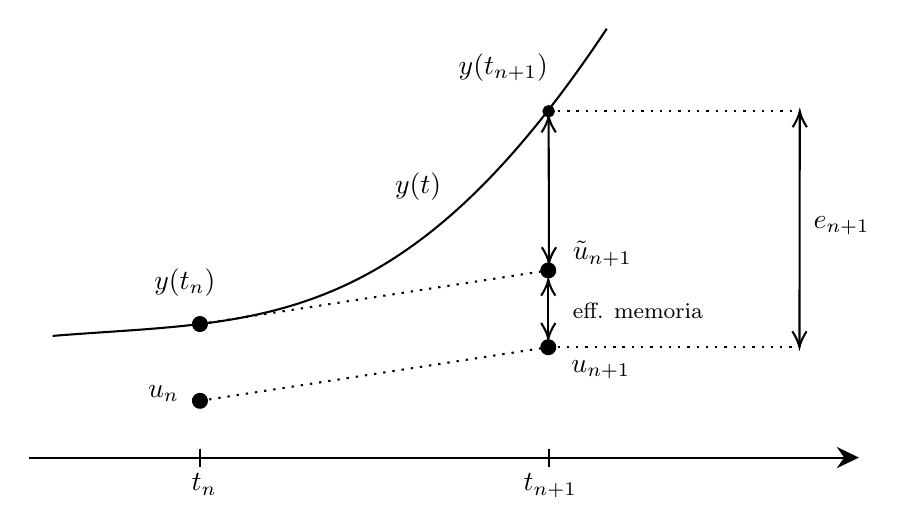
\begin{tikzpicture}[x=0.75pt,y=0.75pt,yscale=-1,xscale=1]
	%uncomment if require: \path (0,266); %set diagram left start at 0, and has height of 266

	%Curve Lines [id:da034892312278599125]
	\draw    (105.5,166.38) .. controls (204.5,158.38) and (273.5,167.38) .. (372.5,18.38) ;
	%Straight Lines [id:da8785454944361366]
	\draw    (176.5,220.67) -- (176.5,229.33) ;
	%Straight Lines [id:da39528602977210503]
	\draw    (94,225) -- (491,225) ;
	\draw [shift={(494,225)}, rotate = 180] [fill={rgb, 255:red, 0; green, 0; blue, 0 }  ][line width=0.08]  [draw opacity=0] (10.72,-5.15) -- (0,0) -- (10.72,5.15) -- (7.12,0) -- cycle    ;
	%Straight Lines [id:da5584172062463073]
	\draw  [dash pattern={on 0.84pt off 2.51pt}]  (176.5,197.67) -- (344.33,171.83) ;
	\draw [shift={(344.33,171.83)}, rotate = 351.25] [color={rgb, 255:red, 0; green, 0; blue, 0 }  ][fill={rgb, 255:red, 0; green, 0; blue, 0 }  ][line width=0.75]      (0, 0) circle [x radius= 3.35, y radius= 3.35]   ;
	\draw [shift={(176.5,197.67)}, rotate = 351.25] [color={rgb, 255:red, 0; green, 0; blue, 0 }  ][fill={rgb, 255:red, 0; green, 0; blue, 0 }  ][line width=0.75]      (0, 0) circle [x radius= 3.35, y radius= 3.35]   ;
	%Straight Lines [id:da2873454849651973]
	\draw  [dash pattern={on 0.84pt off 2.51pt}]  (176.5,160.67) -- (344.33,134.83) ;
	\draw [shift={(344.33,134.83)}, rotate = 351.25] [color={rgb, 255:red, 0; green, 0; blue, 0 }  ][fill={rgb, 255:red, 0; green, 0; blue, 0 }  ][line width=0.75]      (0, 0) circle [x radius= 3.35, y radius= 3.35]   ;
	\draw [shift={(176.5,160.67)}, rotate = 351.25] [color={rgb, 255:red, 0; green, 0; blue, 0 }  ][fill={rgb, 255:red, 0; green, 0; blue, 0 }  ][line width=0.75]      (0, 0) circle [x radius= 3.35, y radius= 3.35]   ;
	%Shape: Circle [id:dp4537649989697854]
	\draw  [fill={rgb, 255:red, 0; green, 0; blue, 0 }  ,fill opacity=1 ] (342,58.17) .. controls (342,56.79) and (343.12,55.67) .. (344.5,55.67) .. controls (345.88,55.67) and (347,56.79) .. (347,58.17) .. controls (347,59.55) and (345.88,60.67) .. (344.5,60.67) .. controls (343.12,60.67) and (342,59.55) .. (342,58.17) -- cycle ;
	%Straight Lines [id:da8554308299700688]
	\draw    (344.5,221) -- (344.5,229.67) ;
	%Straight Lines [id:da6369204585664499]
	\draw    (344.5,62.67) -- (344.66,129.33) ;
	\draw [shift={(344.67,131.33)}, rotate = 269.86] [color={rgb, 255:red, 0; green, 0; blue, 0 }  ][line width=0.75]    (7.65,-3.43) .. controls (4.86,-1.61) and (2.31,-0.47) .. (0,0) .. controls (2.31,0.47) and (4.86,1.61) .. (7.65,3.43)   ;
	\draw [shift={(344.5,60.67)}, rotate = 89.86] [color={rgb, 255:red, 0; green, 0; blue, 0 }  ][line width=0.75]    (7.65,-3.43) .. controls (4.86,-1.61) and (2.31,-0.47) .. (0,0) .. controls (2.31,0.47) and (4.86,1.61) .. (7.65,3.43)   ;
	%Straight Lines [id:da6756464042840566]
	\draw    (344.33,141.33) -- (344.33,165.83) ;
	\draw [shift={(344.33,167.83)}, rotate = 270] [color={rgb, 255:red, 0; green, 0; blue, 0 }  ][line width=0.75]    (7.65,-3.43) .. controls (4.86,-1.61) and (2.31,-0.47) .. (0,0) .. controls (2.31,0.47) and (4.86,1.61) .. (7.65,3.43)   ;
	\draw [shift={(344.33,139.33)}, rotate = 90] [color={rgb, 255:red, 0; green, 0; blue, 0 }  ][line width=0.75]    (7.65,-3.43) .. controls (4.86,-1.61) and (2.31,-0.47) .. (0,0) .. controls (2.31,0.47) and (4.86,1.61) .. (7.65,3.43)   ;
	%Straight Lines [id:da9675193989338564]
	\draw    (465.5,60.17) -- (465.34,169.83) ;
	\draw [shift={(465.33,171.83)}, rotate = 270.08] [color={rgb, 255:red, 0; green, 0; blue, 0 }  ][line width=0.75]    (7.65,-3.43) .. controls (4.86,-1.61) and (2.31,-0.47) .. (0,0) .. controls (2.31,0.47) and (4.86,1.61) .. (7.65,3.43)   ;
	\draw [shift={(465.5,58.17)}, rotate = 90.08] [color={rgb, 255:red, 0; green, 0; blue, 0 }  ][line width=0.75]    (7.65,-3.43) .. controls (4.86,-1.61) and (2.31,-0.47) .. (0,0) .. controls (2.31,0.47) and (4.86,1.61) .. (7.65,3.43)   ;
	%Straight Lines [id:da8189986399115188]
	\draw  [dash pattern={on 0.84pt off 2.51pt}]  (344.33,171.83) -- (465.33,171.83) ;
	%Straight Lines [id:da4540415193091536]
	\draw  [dash pattern={on 0.84pt off 2.51pt}]  (344.5,58.17) -- (465.5,58.17) ;

	% Text Node
	\draw (331,231.4) node [anchor=north west][inner sep=0.75pt]    {$t_{n+1}$};
	% Text Node
	\draw (171,231.4) node [anchor=north west][inner sep=0.75pt]    {$t_{n}$};
	% Text Node
	\draw (354,176.73) node [anchor=north west][inner sep=0.75pt]    {$u_{n+1}$};
	% Text Node
	\draw (299.67,28.73) node [anchor=north west][inner sep=0.75pt]    {$y( t_{n+1})$};
	% Text Node
	\draw (153,132.4) node [anchor=north west][inner sep=0.75pt]    {$y( t_{n})$};
	% Text Node
	\draw (150,188.73) node [anchor=north west][inner sep=0.75pt]    {$u_{n}$};
	% Text Node
	\draw (269,86.4) node [anchor=north west][inner sep=0.75pt]    {$y(t)$};
	% Text Node
	\draw (354.67,149) node [anchor=north west][inner sep=0.75pt]  [font=\footnotesize] [align=left] {eff. memoria};
	% Text Node
	\draw (354.67,119.4) node [anchor=north west][inner sep=0.75pt]    {$\tilde{u}_{n+1}$};
	% Text Node
	\draw (470.67,107.4) node [anchor=north west][inner sep=0.75pt]    {$e_{n+1}$};
	\end{tikzpicture}
	\caption{Intuizione grafica del ruolo dell'errore di consistenza e dell'effetto memoria nell'analisi di convergenza del metodo di Eulero Esplicito.}
\end{figure}

Dobbiamo stimare separatamente questi due errori.
\begin{enumerate}
\item Stimiamo l'errore di consistenza $y( t_{n+1}) -\tilde{u}_{n+1}$.

Scriviamo lo sviluppo di Taylor di $y$:
\begin{equation*}
y( t_{n+1}) =y( t_{n}) +hy'( t_{n}) +\frac{h^{2}}{2} y''( \xi ) ,\quad \xi \in ( t_{n} ,t_{n+1})
\end{equation*}
e sostituiamola insieme a \eqref{eq:convergenza-ee-primo-passo}:
\begin{align*}
y( t_{n+1}) -\tilde{u}_{n+1} & =\cancel{y( t_{n})} +\cancel{hf( t_{n} ,y( t_{n}))} +\frac{h^{2}}{2} y''( \xi ) -\cancel{y( t_{n})} -\cancel{hf( t_{n} ,y( t_{n}))}\\
 & =\frac{h^{2}}{2} y''( \xi ) =h\tau _{n+1}(h).
\end{align*}
\item Stimiamo l'errore dovuto all'effetto memoria, $\tilde{u}_{n+1} -u_{n+1}$:
\begin{align*}
	\tilde{u}_{n+1}                        & =y( t_{n}) +hf( t_{n} ,y( t_{n}))                                                  &                           \\
	u_{n+1}                                & =u_{n} +hf( t_{n} ,u_{n})                                                          &                           \\
	\tilde{u}_{n+1} -u_{n+1}               & =\underbrace{y( t_{n}) -u_{n}}_{e_{n}} +h[ f( t_{n} ,y( t_{n})) -f( t_{n} ,u_{n})] & \text{(sottraiamo)}       \\
	\left| \tilde{u}_{n+1} -u_{n+1}\right| & \leqslant | e_{n}| +h| f( t_{n} ,y( t_{n})) -f( t_{n} ,u_{n})|                     & \text{(modulo)}           \\
	                                       & \leqslant | e_{n}| +hL\underbrace{| y( t_{n}) -u_{n}| }_{e_{n}}                    & \text{(lipschitzianità)} \\
	                                       & \leqslant ( 1+hL)| e_{n}|.                                                         &
\end{align*}
\end{enumerate}
Mettendo insieme le due stime troviamo:
\begin{equation*}
| e_{n+1}| \leqslant h\tau _{n+1}(h) +( 1+hL)| e_{n}|
\end{equation*}
che possiamo riscrivere come:
\begin{equation*}
\begin{aligned}
| e_{n+1}|  & \leqslant h\tau (h) +( 1+hL)| e_{n}| \\
 & \leqslant h\tau (h) +( 1+hL)[ h\tau (h) +( 1+hL)| e_{n-1}| ]\\
 & \vdots \ ( e_{0} =0)\\
 & \leqslant h\tau (h)\left[ 1+( 1+hL) +( 1+hL)^{2} +\cdots +( 1+hL)^{n}\right]\\
 & \leqslant h\tau (h)\sum\limits ^{n}_{k=0}( 1+hL)^{k}
\end{aligned}
\end{equation*}
ricordando che $\tau (h) =\frac{h}{2}\Vert y''(t)\Vert _{\infty }$.
Sfruttiamo ora l'espressione della serie geometrica
\begin{equation*}
\sum\limits ^{n}_{k=0} x^{k} =\frac{1-x^{k+1}}{1-x},
\end{equation*}
pertanto abbiamo che
\begin{align*}
| e_{n+1}|  & \leqslant h\tau (h)\left[\frac{1-( 1+hL)^{n+1}}{1-( 1+hL)}\right]\\
 & \leqslant \frac{\tau (h)}{L}\left[ -1+( 1+hL)^{n+1}\right]\\
 & \leqslant \frac{\left[ e^{( n+1) hL} -1\right]}{L} \tau (h)\\
 & \leqslant \frac{e^{TL}}{L} \tau (h),
\end{align*}
allora il metodo converge perché $\tau (h) =\frac{h}{2}\Vert y''(t)\Vert _{\infty }$ e:
\begin{equation*}
| e_{n+1}| \leqslant Ch,\quad C=\frac{e^{TL}}{2L}\Vert y''(t)\Vert _{\infty } ,\quad \forall n=0,\dotsc ,N_{h} -1.
\end{equation*}
L'ordine di convergenza è $1$. \textqed

% \textit{[Lezione 19 (5-05-2020)]}
Riassumiamo senza dimostrare i risultati di convergenza di tutti e quattro i metodi studiati.
\begin{theorem}
[Convergenza di \eqref{eq:eulero-avanti}, \eqref{eq:eulero-indietro}, \eqref{eq:crank-nicolson}, \eqref{eq:heun}]
Sia $y\in C^{2}(I)$ la soluzione del \eqref{eq:problema-di-cauchy}. Allora
\begin{gather*}
\max_{n=0,\dotsc ,N_{h}}\left| y( t_{n}) -u^{EE}_{n}\right| \leqslant C_{EE} h\\
\max_{n=0,\dotsc ,N_{h}}\left| y( t_{n}) -u^{EI}_{n}\right| \leqslant C_{EI} h
\end{gather*}
dove $C_{EE} =C_{EE}(\Vert y''(t)\Vert _{\infty } ,T)  >0$ e $C_{EI} =C_{EI}(\Vert y''(t)\Vert _{\infty } ,T)  >0$. Quindi i metodi di \eqref{eq:eulero-avanti} e \eqref{eq:eulero-indietro} convergono con ordine $1$ rispetto ad $h$.

Se invece $y\in C^{3}(I)$, allora
\begin{gather*}
\max_{n=0,\dotsc ,N_{h}}\left| y( t_{n}) -u^{CN}_{n}\right| \leqslant C_{CN} h^{2}\\
\max_{n=0,\dotsc ,N_{h}}\left| y( t_{n}) -u^{H}_{n}\right| \leqslant C_{H} h^{2}
\end{gather*}
dove $C_{CN} =C_{CN}(\Vert y'''(t)\Vert _{\infty } ,T)  >0$ e $C_{H} =C_{H}(\Vert y'''(t)\Vert _{\infty } ,T)  >0$. Quindi i metodi di \eqref{eq:crank-nicolson} e \eqref{eq:heun} convergono con ordine $2$ rispetto ad $h$.
\end{theorem}

\subsection{Assoluta stabilità}
Studiamo il comportamento dei metodi quando $h$ è fissato e $t_{n}\rightarrow \infty $: in tal caso, desideriamo che la soluzione numerica $u_{n}$ si mantenga \textit{vicina} a $y( t_{n})$. Questa caratteristica è nota come \textbf{assoluta stabilità}\index{assoluta stabilità}, o $\mathcal{A}$\textbf{-stabilità}\index{$\mathcal{A}$-stabilità}.

Per analizzare la stabilità su intervalli illimitati, considereremo il seguente \textit{problema modello}:
\begin{equation}\tag{PMod}
\begin{cases}
y'(t) =\lambda y(t) ,\quad t\in ( 0,+\infty )\\
y(0) =1
\end{cases}
\label{eq:problema-modello}
\end{equation}
con $\lambda \in \mathbb{C}$, la cui soluzione di è $y(t) =e^{\lambda t}$. Inoltre se $\Re ( \lambda ) < 0$, si ha che $$\lim\limits _{t\rightarrow +\infty }| y(t)| =0.$$

\fg[Comportamento di \eqref{eq:problema-modello}]{0.7}{fig-problema-modello}

Vorremmo dunque che anche la soluzione numerica tenda a zero, in modo da catturare il comportamento asintotico della soluzione vera.
\begin{definition}
[Assoluta stabilità]
\index{assoluta stabilità}
Diciamo che un metodo numerico per l'approssimazione di \eqref{eq:problema-modello} è assolutamente stabile se
\begin{equation}
| u_{n}| \rightarrow 0\quad \text{per} \quad t_{n}\rightarrow +\infty.
\end{equation}
\label{eq:assoluta-stabilita}
\end{definition}

\textit{Osservazione.}
Per $h$ fissato, la soluzione numerica $u_{n}$ dipende da $h$ e da $\lambda $. Possiamo quindi dare la seguente definizione.
\begin{definition}
[Regione di assoluta stabilità]
\index{regione di assoluta stabilità}
Definiamo $\mathcal{A}$ la regione di assoluta stabilità di un metodo numerico il seguente sottoinsieme del piano complesso:
$$\mathcal{A} =\{z=h\lambda \in \mathbb{C} \text{ tali che \eqref{eq:assoluta-stabilita} è soddisfatta}\}.$$
\end{definition}

\textbf{NB.}
Poiché $h >0$ e $\Re ( \lambda ) < 0$ per ipotesi, sicuramente $\mathcal{A} \subseteq \mathbb{C}^{-}$.

\begin{definition}
[$\mathcal{A}$-stabilità]
\index{$\mathcal{A}$-stabilità}
Un metodo numerico è $\mathcal{A}$-stabile se $\mathcal{A} \cap \mathbb{C}^{-} =\mathbb{C}^{-}$, ovvero se per qualsiasi $\lambda \in \mathbb{C}^{-}$ la condizione \eqref{eq:assoluta-stabilita} è soddisfatta incondizionatamente rispetto ad $h$.
\end{definition}

\subsection{Stabilità di Eulero Esplicito}
Il metodo di Eulero esplicito applicato al problema modello \eqref{eq:problema-modello} diventa:
\begin{equation*}
\begin{cases}
u_{n+1} =u_{n} +h\underbrace{\lambda u_{n}}_{f( t_{n} ,u_{n})} \quad n=0,1,2,\dotsc \\
u_{0} =1.
\end{cases}
\end{equation*}
Quindi otteniamo $u_{n+1} =( 1+h\lambda ) u_{n}$, cioè, ricorsivamente:
\begin{align*}
u_{n+1} & =( 1+h\lambda ) u_{n}\\
 & =( 1+h\lambda )( 1+h\lambda ) u_{n-1}\\
 & \vdots \\
 & =( 1+h\lambda )^{n+1} u_{0}\\
 & =( 1+h\lambda )^{n+1}.
\end{align*}
Abbiamo quindi mostrato che il metodo di \eqref{eq:eulero-avanti} utilizzato per approssimare \eqref{eq:problema-modello} ha la seguente forma:
\begin{equation*}
\begin{cases}
u_{n} =( 1+h\lambda )^{n} \quad n=0,1,2,\dotsc \\
u_{0} =1.
\end{cases}
\end{equation*}
Dalla definizione di assoluta stabilità si ha che:
\begin{align}
\lim _{t_{n}\rightarrow +\infty }| u_{n}| =0 \quad  & \Leftrightarrow \quad\lim _{t_{n}\rightarrow +\infty }\left| ( 1+h\lambda )^{n}\right| =0\Leftrightarrow | 1+h\lambda | < 1 \\
													& \Leftrightarrow \quad h\lambda \in \mathbb{C}^{-} \ \text{e} \ 0< h< \frac{-2\Re ( \lambda )}{| \lambda | ^{2}}.
\label{eq:A-stab-ee}
\end{align}

\begin{figure}[htpb]
	\centering
	\tikzset{
	pattern size/.store in=\mcSize,
	pattern size = 5pt,
	pattern thickness/.store in=\mcThickness,
	pattern thickness = 0.3pt,
	pattern radius/.store in=\mcRadius,
	pattern radius = 1pt}
	\makeatletter
	\pgfutil@ifundefined{pgf@pattern@name@_abw8ptezs}{
	\pgfdeclarepatternformonly[\mcThickness,\mcSize]{_abw8ptezs}
	{\pgfqpoint{0pt}{-\mcThickness}}
	{\pgfpoint{\mcSize}{\mcSize}}
	{\pgfpoint{\mcSize}{\mcSize}}
	{
	\pgfsetcolor{\tikz@pattern@color}
	\pgfsetlinewidth{\mcThickness}
	\pgfpathmoveto{\pgfqpoint{0pt}{\mcSize}}
	\pgfpathlineto{\pgfpoint{\mcSize+\mcThickness}{-\mcThickness}}
	\pgfusepath{stroke}
	}}
	\makeatother
	\tikzset{every picture/.style={line width=0.75pt}} %set default line width to 0.75pt

	\begin{tikzpicture}[x=0.75pt,y=0.75pt,yscale=-1,xscale=1]
	%uncomment if require: \path (0,198); %set diagram left start at 0, and has height of 198

	%Shape: Axis 2D [id:dp6880840645767705]
	\draw  (166.03,112.08) -- (426.53,112.08)(296.5,41.65) -- (296.5,184.57) (419.53,107.08) -- (426.53,112.08) -- (419.53,117.08) (291.5,48.65) -- (296.5,41.65) -- (301.5,48.65)  ;
	%Shape: Circle [id:dp9444959892220257]
	\draw  [pattern=_abw8ptezs,pattern size=3.75pt,pattern thickness=0.75pt,pattern radius=0pt, pattern color={rgb, 255:red, 155; green, 155; blue, 155}] (209.5,112.08) .. controls (209.5,88.05) and (228.98,68.58) .. (253,68.58) .. controls (277.02,68.58) and (296.5,88.05) .. (296.5,112.08) .. controls (296.5,136.1) and (277.02,155.58) .. (253,155.58) .. controls (228.98,155.58) and (209.5,136.1) .. (209.5,112.08) -- cycle ;

	% Text Node
	\draw (439,103.4) node [anchor=north west][inner sep=0.75pt]    {$\Re ( h\lambda )$};
	% Text Node
	\draw (275,15.4) node [anchor=north west][inner sep=0.75pt]    {$\Im ( h\lambda )$};
	% Text Node
	\draw (181,115.4) node [anchor=north west][inner sep=0.75pt]    {$-2$};


	\end{tikzpicture}
	\caption{Regione di stabilità di \eqref{eq:eulero-avanti}. Si notino in particolare gli assi che sono la parte reale e immaginaria di $h\lambda$.}
\end{figure}

Ovvero abbiamo mostrato che \eqref{eq:eulero-avanti} è assolutamente stabile solo sotto queste condizioni.
Si dice quindi che il metodo di \eqref{eq:eulero-avanti} è \textit{condizionatamente assolutamente stabile}.

\textit{Osservazione.} Se $\lambda \in \mathbb{R} ,\lambda < 0$ allora \eqref{eq:A-stab-ee} diventa $h< 2/| \lambda |$.

\subsection{Stabilità di Eulero Implicito}
Discretizziamo ora \eqref{eq:problema-modello} con il metodo di \eqref{eq:eulero-indietro}:
\begin{equation*}
\begin{cases}
u_{n+1} =u_{n} +h\lambda u_{n+1} \quad n=0,1,2,\dotsc \\
u_{0} =1
\end{cases}
\end{equation*}
da cui otteniamo $u_{0} =1$ e $( 1-h\lambda ) u_{n+1} =u_{n}$ e quindi:
\begin{equation*}
\begin{cases}
u_{n+1} =\frac{1}{( 1-h\lambda )} u_{n} \quad n=0,1,2,\dotsc \\
u_{0} =1,
\end{cases}
\end{equation*}
ragionando ricorsivamente come prima $u_{n+1} =\frac{1}{( 1-h\lambda )^{n+1}}$. Dunque:
\begin{equation*}
\lim _{t_{n}\rightarrow +\infty }| u_{n}| =0\Leftrightarrow \lim _{t_{n}\rightarrow +\infty }\left| \frac{1}{( 1-h\lambda )^{n}}\right| =0\Leftrightarrow \left| \frac{1}{( 1-h\lambda )^{n}}\right| < 1\Leftrightarrow | 1-h\lambda |  >1.
\end{equation*}

\begin{figure}[htpb]
	\centering
	\tikzset{
	pattern size/.store in=\mcSize,
	pattern size = 5pt,
	pattern thickness/.store in=\mcThickness,
	pattern thickness = 0.3pt,
	pattern radius/.store in=\mcRadius,
	pattern radius = 1pt}
	\makeatletter
	\pgfutil@ifundefined{pgf@pattern@name@_va1vrgvkr}{
	\pgfdeclarepatternformonly[\mcThickness,\mcSize]{_va1vrgvkr}
	{\pgfqpoint{0pt}{-\mcThickness}}
	{\pgfpoint{\mcSize}{\mcSize}}
	{\pgfpoint{\mcSize}{\mcSize}}
	{
	\pgfsetcolor{\tikz@pattern@color}
	\pgfsetlinewidth{\mcThickness}
	\pgfpathmoveto{\pgfqpoint{0pt}{\mcSize}}
	\pgfpathlineto{\pgfpoint{\mcSize+\mcThickness}{-\mcThickness}}
	\pgfusepath{stroke}
	}}
	\makeatother

	% Pattern Info

	\tikzset{
	pattern size/.store in=\mcSize,
	pattern size = 5pt,
	pattern thickness/.store in=\mcThickness,
	pattern thickness = 0.3pt,
	pattern radius/.store in=\mcRadius,
	pattern radius = 1pt}
	\makeatletter
	\pgfutil@ifundefined{pgf@pattern@name@_r9v1a7k8k}{
	\pgfdeclarepatternformonly[\mcThickness,\mcSize]{_r9v1a7k8k}
	{\pgfqpoint{0pt}{0pt}}
	{\pgfpoint{\mcSize+\mcThickness}{\mcSize+\mcThickness}}
	{\pgfpoint{\mcSize}{\mcSize}}
	{
	\pgfsetcolor{\tikz@pattern@color}
	\pgfsetlinewidth{\mcThickness}
	\pgfpathmoveto{\pgfqpoint{0pt}{0pt}}
	\pgfpathlineto{\pgfpoint{\mcSize+\mcThickness}{\mcSize+\mcThickness}}
	\pgfusepath{stroke}
	}}
	\makeatother
	\tikzset{every picture/.style={line width=0.75pt}} %set default line width to 0.75pt

	\begin{tikzpicture}[x=0.75pt,y=0.75pt,yscale=-1,xscale=1]
	%uncomment if require: \path (0,198); %set diagram left start at 0, and has height of 198

	%Shape: Rectangle [id:dp7375440624549783]
	\draw  [draw opacity=0][pattern=_va1vrgvkr,pattern size=3.75pt,pattern thickness=0.75pt,pattern radius=0pt, pattern color={rgb, 255:red, 155; green, 155; blue, 155}] (167,50.53) -- (417.5,50.53) -- (417.5,183.53) -- (167,183.53) -- cycle ;
	%Shape: Circle [id:dp02186694773818809]
	\draw  [fill={rgb, 255:red, 255; green, 255; blue, 255 }  ,fill opacity=1 ] (296.5,112.08) .. controls (296.5,88.05) and (315.98,68.58) .. (340,68.58) .. controls (364.02,68.58) and (383.5,88.05) .. (383.5,112.08) .. controls (383.5,136.1) and (364.02,155.58) .. (340,155.58) .. controls (315.98,155.58) and (296.5,136.1) .. (296.5,112.08) -- cycle ;
	%Shape: Rectangle [id:dp8854778510306025]
	\draw  [draw opacity=0][pattern=_r9v1a7k8k,pattern size=3.75pt,pattern thickness=0.75pt,pattern radius=0pt, pattern color={rgb, 255:red, 155; green, 155; blue, 155}] (167,50.53) -- (297.25,50.53) -- (297.25,183.53) -- (167,183.53) -- cycle ;
	%Shape: Axis 2D [id:dp7471649485705765]
	\draw  (166.03,112.08) -- (426.53,112.08)(296.5,41.65) -- (296.5,184.57) (419.53,107.08) -- (426.53,112.08) -- (419.53,117.08) (291.5,48.65) -- (296.5,41.65) -- (301.5,48.65)  ;

	% Text Node
	\draw (439,103.4) node [anchor=north west][inner sep=0.75pt]    {$\Re ( h\lambda )$};
	% Text Node
	\draw (275,15.4) node [anchor=north west][inner sep=0.75pt]    {$\Im ( h\lambda )$};
	% Text Node
	\draw (366,113.4) node [anchor=north west][inner sep=0.75pt]    {$2$};


	\end{tikzpicture}
	\caption{Regione di stabilità di \eqref{eq:eulero-indietro}. L'intersezione tra il complementare del cerchio e il semipiano di sinistra è proprio il semipiano di sinistra, da cui l'assoluta stabilità.}
\end{figure}
\FloatBarrier

Il metodo di \eqref{eq:eulero-indietro} è assolutamente stabile senza condizioni su $h$ perché ci interessa solo la parte negativa del piano complesso, essendo $h >0$ e $\Re ( \lambda ) < 0$.
In altre parole, il metodo di \eqref{eq:eulero-indietro} è $\mathcal{A}$-stabile.

Ecco perché in certe occasioni, quando il dominio dell'equazione differenziale è molto ampio, i metodi impliciti sono più convenienti, pur essendo più costosi.


\subsection{Stabilità di Crank-Nicolson e Heun}
Discretizzando \eqref{eq:problema-modello} con il metodo di \eqref{eq:crank-nicolson} otteniamo:
\begin{equation*}\tag{CN'} % Ho aggiunto un ' per la discretizzazione
\begin{cases}
u_{n+1} =\left[\frac{\left( 1+\frac{h\lambda }{2}\right)}{\left( 1-\frac{h\lambda }{2}\right)}\right]^{n+1} n\geqslant 0\\
u_{0} =1
\end{cases}
\end{equation*}
che si rivela quindi $\mathcal{A}$-stabile. Invece per \eqref{eq:heun} otteniamo:
\begin{equation*}\tag{H'} % Ho aggiunto un ' per la discretizzazione
\begin{cases}
u_{n+1} =\left[ 1+h\lambda +\frac{( h\lambda )^{2}}{2}\right]^{n+1} n\geqslant 0\\
u_{0} =1.
\end{cases}
\end{equation*}
Esso è dunque condizionatamente assolutamente stabile. La regione di stabilità per \eqref{eq:heun} è rappresenta in figura \ref{fig:stabilita-heun}.

\begin{figure}[htpb]
	\centering
	\tikzset{
	pattern size/.store in=\mcSize,
	pattern size = 5pt,
	pattern thickness/.store in=\mcThickness,
	pattern thickness = 0.3pt,
	pattern radius/.store in=\mcRadius,
	pattern radius = 1pt}
	\makeatletter
	\pgfutil@ifundefined{pgf@pattern@name@_bycubmjjm}{
	\pgfdeclarepatternformonly[\mcThickness,\mcSize]{_bycubmjjm}
	{\pgfqpoint{0pt}{-\mcThickness}}
	{\pgfpoint{\mcSize}{\mcSize}}
	{\pgfpoint{\mcSize}{\mcSize}}
	{
	\pgfsetcolor{\tikz@pattern@color}
	\pgfsetlinewidth{\mcThickness}
	\pgfpathmoveto{\pgfqpoint{0pt}{\mcSize}}
	\pgfpathlineto{\pgfpoint{\mcSize+\mcThickness}{-\mcThickness}}
	\pgfusepath{stroke}
	}}
	\makeatother
	\tikzset{every picture/.style={line width=0.75pt}} %set default line width to 0.75pt

	\begin{tikzpicture}[x=0.75pt,y=0.75pt,yscale=-1,xscale=1]
	%uncomment if require: \path (0,227); %set diagram left start at 0, and has height of 227

	%Shape: Axis 2D [id:dp40882529573161475]
	\draw  (146.03,124.79) -- (406.53,124.79)(276.5,34.31) -- (276.5,217.9) (399.53,119.79) -- (406.53,124.79) -- (399.53,129.79) (271.5,41.31) -- (276.5,34.31) -- (281.5,41.31)  ;
	%Shape: Ellipse [id:dp47835041184589744]
	\draw  [pattern=_bycubmjjm,pattern size=3.75pt,pattern thickness=0.75pt,pattern radius=0pt, pattern color={rgb, 255:red, 155; green, 155; blue, 155}] (189.5,125.08) .. controls (189.5,89.86) and (208.98,61.31) .. (233,61.31) .. controls (257.02,61.31) and (276.5,89.86) .. (276.5,125.08) .. controls (276.5,160.29) and (257.02,188.84) .. (233,188.84) .. controls (208.98,188.84) and (189.5,160.29) .. (189.5,125.08) -- cycle ;
	%Straight Lines [id:da6650487688260662]
	\draw  [dash pattern={on 0.84pt off 2.51pt}]  (276.5,61.31) -- (233,61.31) ;
	%Straight Lines [id:da15173594668774437]
	\draw  [dash pattern={on 0.84pt off 2.51pt}]  (276.5,188.84) -- (233,188.84) ;

	% Text Node
	\draw (419,116.4) node [anchor=north west][inner sep=0.75pt]    {$\Re ( h\lambda )$};
	% Text Node
	\draw (256,9.4) node [anchor=north west][inner sep=0.75pt]    {$\Im ( h\lambda )$};
	% Text Node
	\draw (161,128.4) node [anchor=north west][inner sep=0.75pt]    {$-2$};
	% Text Node
	\draw (283,53.4) node [anchor=north west][inner sep=0.75pt]    {$1.75$};
	% Text Node
	\draw (283,180.4) node [anchor=north west][inner sep=0.75pt]    {$-1.75$};


	\end{tikzpicture}
	\caption{Regione di stabilità per \eqref{eq:heun}.}
	\label{fig:stabilita-heun}
\end{figure}

\textit{Osservazioni.}
\begin{enumerate}
\item Si può dimostrare che un metodo esplicito non può essere $\mathcal{A}$-stabile, cioè tutti i metodi espliciti sono condizionatamente assolutamente stabili: esiste sempre una qualche condizione su $h\lambda $.
Come spesso succede, si ha quindi un trade-off tra efficienza computazionale (metodi espliciti) e stabilità dell'approssimazione (metodi impliciti).
\item Non tutti i metodi impliciti sono $\mathcal{A}$-stabili.
\end{enumerate}

\subsection{Tabella riassuntiva}
\begin{center}

\begin{tabular}{ccccc}
\toprule
  & Consistenza & Zero-stabilità & Ordine di convergenza & Assoluta stabilità \\
\midrule
\eqref{eq:eulero-avanti} & sì & sì & $h$ & condiz. ass. stabile \\
\eqref{eq:eulero-indietro} & sì & sì & $h$ & $\mathcal{A}$-stabile \\
\eqref{eq:crank-nicolson} & sì & sì & $h^{2}$ & $\mathcal{A}$-stabile \\
\eqref{eq:heun} & sì & sì & $h^{2}$ & condiz. ass. stabile \\
 \bottomrule
\end{tabular}
\end{center}
Nel seguito vedremo due macro-famiglie di metodi numerici di ordine elevato per EDO:
\begin{itemize}
\item \textbf{Metodi di Runge-Kutta}\index{metodo!di Runge-Kutta} (a $1$ passo): per aumentare l'ordine di convergenza si utilizzano delle valutazioni aggiuntive di $f$ tra $t_{n}$ e $t_{n+1}$.
\item \textbf{Metodi multistep}\index{metodo!multistep} (a $p$ passi): l'ordine di convergenza è legato al numero di passi utilizzati.
\end{itemize}
\section{Metodi di Runge-Kutta}

Partiamo ancora una volta dal problema di Cauchy \eqref{eq:problema-di-cauchy}.
I metodi di Runge-Kutta hanno la seguente forma:
\begin{equation}
\begin{cases}
u_{n+1} =u_{n} +h\sum\limits ^{s}_{i=1} b_{i} K_{i} \qquad \text{con } n\geqslant 0\\
u_{0} =y_{0},
\end{cases}
\end{equation}
dove $s$ è detto \textbf{numero di stadi}\index{numero di stadi} del metodo, ed è legato all'ordine del metodo.

I coefficienti $K_{i}$ sono le valutazioni non solo in $t_{n}$ e $t_{n+1}$ ma anche in punti intermedi:
\begin{equation}
K_{i} =f\left( t_{n} +c_{i} h,u_{n} +h\sum\limits ^{s}_{j=1} a_{ij} K_{j}\right) ,\quad i=1,\dotsc ,s.
\end{equation}
I coefficienti $\{a_{ij}\}_{i,j=1,\dotsc ,s}$, $\{b_{i}\}_{i=1,\dotsc ,s}$ e $\{c_{i}\}_{i=1,\dotsc ,s}$ sono memorizzati nell'\textit{array di Butcher} e caratterizzano univocamente il particolare metodo di RK utilizzato:
\begin{equation}
\begin{array}{ c|c c c c }
c_{1} & a_{11} & a_{12} & \cdots  & a_{1s}\\
c_{2} & a_{21} & a_{22} & \cdots  & a_{2s}\\
\vdots  & \vdots  & \vdots  & \ddots  & \vdots \\
c_{s} & a_{s1} & a_{s2} & \cdots  & a_{ss}\\
\hline
 & b_{1} & b_{2} & \cdots  & b_{s}
\end{array} \quad \text{o} \quad \begin{array}{ c|c }
\mathbf{c} & A\\
\hline
 & \mathbf{b}^{T}
\end{array}
\end{equation}
Come suggerito dalla notazione, i vincoli applicati a questi coefficienti sono:
\begin{equation}
c_{i} =\sum\limits ^{s}_{j=1} a_{ij} ,\quad \sum\limits ^{s}_{i=1} b_{i} =1,\quad i=1,\dotsc ,s.
\end{equation}
\label{eq:ipotesi-rk}
Vedremo nel teorema \ref{thm:metodo-rk-consistente} che la condizione su $b$ serve a garantire un'importante proprietà del metodo.

\subsection{Classificazione dei metodi Runge-Kutta}
I metodi di RK si possono classificare nel seguente modo:
\begin{itemize}
\item \textbf{RK espliciti}\index{metodo!di Runge-Kutta esplicito} $: a_{ij} =0 \ \forall j\geqslant i)$. $K_{i}$ può essere calcolato a partire da $K_{1} ,K_{2} ,\dotsc ,K_{i-1}$.
\begin{equation*}
\begin{array}{ c|c c c c }
c_{1} & 0 & 0 & \cdots  & 0\\
c_{2} & a_{21} & 0 & \cdots  & 0\\
\vdots  & \vdots  & \vdots  & \ddots  & \vdots \\
c_{s} & a_{s1} & a_{s2} & \cdots  & 0\\
\hline
 & b_{1} & b_{2} & \cdots  & b_{s}
\end{array}
\end{equation*}

\item \textbf{RK semi-impliciti}\index{metodo!di Runge-Kutta semi-implicito} $: a_{ij} =0 \ \forall j >i)$. $K_{i}$ dipende non linearmente solo da sé stesso. Abbiamo un sistema di $s$ equazioni non-lineari disaccoppiate in $K_{1} ,\dotsc ,k_{s}$.
\begin{equation*}
\begin{array}{ c|c c c c }
c_{1} & a_{11} & 0 & \cdots  & 0\\
c_{2} & a_{21} & a_{22} & \cdots  & 0\\
\vdots  & \vdots  & \vdots  & \ddots  & \vdots \\
c_{s} & a_{s1} & a_{s2} & \cdots  & a_{ss}\\
\hline
 & b_{1} & b_{2} & \cdots  & b_{s}
\end{array}
\end{equation*}

\item \textbf{RK impliciti}\index{metodo!di Runge-Kutta implicito}. Non ho restrizioni su $a_{ij}$, abbiamo un sistema di $s$ equazioni non-lineari in $k_{1} ,\dotsc ,k_{s}$.
\begin{equation*}
\begin{array}{ c|c c c c }
c_{1} & a_{11} & a_{12} & \cdots  & a_{1s}\\
c_{2} & a_{21} & a_{22} & \cdots  & a_{2s}\\
\vdots  & \vdots  & \vdots  & \ddots  & \vdots \\
c_{s} & a_{s1} & a_{s2} & \cdots  & a_{ss}\\
\hline
 & b_{1} & b_{2} & \cdots  & b_{s}
\end{array}
\end{equation*}
\end{itemize}
% \textit{[Lezione 20 (11-05-2020)]}

Costruiamo un metodo RK \textit{esplicito} a $s=2$ stadi. Partiamo dalla forma generale:
\begin{equation*}
\begin{cases}
u_{n+1} =u_{n} +h( b_{1} K_{1} +b_{2} K_{2})\\
u_{0} =y_{0},
\end{cases}
\end{equation*}
dove
\begin{equation}
\begin{aligned}
K_{1} =f( t_{n} +c_{1} h,u_{n} +h( a_{11} K_{1} +a_{12} K_{2}))\\
K_{2} =f( t_{n} +c_{2} h,u_{n} +h( a_{21} K_{1} +a_{22} K_{2})).
\end{aligned}
\label{eq:rk-esplicito-2-stadi-passaggio}
\end{equation}
L'array di Butcher risulta:
\begin{equation*}
\begin{array}{ c|c c }
c_{1} & a_{11} & a_{12}\\
c_{2} & a_{21} & a_{22}\\
\hline
 & b_{1} & b_{2}
\end{array}
\end{equation*}
Poiché vogliamo costruire un metodo esplicito, dobbiamo imporre $a_{ij} =0,\forall j\geqslant i$, ovvero
\begin{equation*}
a_{11} =a_{12} =a_{22} =0.
\end{equation*}
Quindi l'array da calcolare diventa:
\begin{equation*}
\begin{array}{ c|c c }
c_{1} & 0 & 0\\
c_{2} & a_{21} & 0\\
\hline
 & b_{1} & b_{2}
\end{array}
\end{equation*}
A questo punto sfruttiamo le ipotesi \eqref{eq:ipotesi-rk}:
\begin{equation*}
\begin{aligned}
\sum\limits ^{s}_{i=1} b_{i} =1 & \Rightarrow b_{1} +b_{2} =1\\
c_{i} =\sum\limits ^{s}_{j=1} a_{ij} & \Rightarrow \begin{cases}
c_{1} =0\\
c_{2} =a_{21}.
\end{cases}
\end{aligned}
\end{equation*}
Allora l'array diventa:
\begin{equation*}
\begin{array}{ c|c c }
0 & 0 & 0\\
c_{2} & c_{2} & 0\\
\hline
 & b_{1} & b_{2}
\end{array} \quad \text{con} \quad b_{1} +b_{2} =1.
\end{equation*}
L'idea per calcolare tali coefficienti è quella di sviluppare in serie di Taylor la soluzione numerica e quella esatta, e imporre l'uguaglianza tra i primi termini di questi sviluppi.
% Svolgendo i conti si ottiene che:
% \begin{equation*}
% \begin{cases}
% b_{1} +b_{2} =1\\
% b_{2} c_{2} =\frac{1}{2}
% \end{cases}
% \end{equation*} % già inclusi più avanti
Riprendiamo l'espressione \eqref{eq:rk-esplicito-2-stadi-passaggio} e il metodo, che diventano:
\begin{equation*}
\begin{array}{ l }
K_{1} =f( t_{n} ,u_{n})\\
K_{2} =f( t_{n} +c_{2} h,u_{n} +hc_{2} K_{1})\\
u_{n+1} =u_{n} +h( b_{1} K_{1} +b_{2} K_{2}).
\end{array}
\end{equation*}
Per calcolare esplicitamente $c_{2} ,b_{1} ,b_{2}$ supponiamo di conoscere la soluzione esatta all'istante $t_{n}$: $y( t_{n}) =y_{n}$. Sviluppiamo in serie di Taylor $K_{2}$ in un intorno di $t_{n}$, arrestandoci al secondo ordine:
\begin{equation*}
\begin{aligned}
K_{2} & =f( t_{n} +c_{2} h,u_{n} +hc_{2} K_{1})\\
 & =f( t_{n} ,y_{n}) +c_{2} h( f_{n,t} +K_{1} f_{n,y}) +O\left( h^{2}\right)
\end{aligned}
\end{equation*}
dove abbiamo usato la notazione
$$ f_{n,t} =\frac{\partial f( t,y)}{\partial t} |_{t=t_{n} ,y=y_{n}} \quad \text{e} \quad f_{n,y} =\frac{\partial f( t,y)}{\partial y} |_{t=t_{n} ,y=y_{n}}, $$
che indicano le derivate parziali di $f$ rispetto a $t$ e $y$ (rispettivamente), e valutata nel punto $( t_{n} ,y_{n})$.

Sostituiamo lo sviluppo nel metodo RK:
\begin{equation}
\begin{aligned}
u^{\star }_{n+1} & =u_{n} +h( b_{1} K_{1} +b_{2} K_{2})\\
 & =y_{n} +h\left( b_{1} f( t_{n} ,y_{n}) +b_{2}\left( f( t_{n} ,y_{n}) +c_{2} h( f_{n,t} +K_{1} f_{n,y}) +O\left( h^{2}\right)\right)\right)\\
 & =y_{n} +h\left( b_{1} f( t_{n} ,y_{n}) +b_{2}\left( f( t_{n} ,y_{n}) +c_{2} h( f_{n,t} +f( t_{n} ,y_{n}) f_{n,y}) +O\left( h^{2}\right)\right)\right).
\end{aligned}
\label{eq:soluzione-rk}
\end{equation}
Analogamente, se sviluppiamo la soluzione esatta in un intorno di $t_{n}$:
\begin{equation}
\begin{aligned}
y_{n+1} & =y_{n} +hy'_{n} +\frac{h^{2}}{2} y''_{n} +O\left( h^{3}\right)\\
 & =y_{n} +hf( t_{n} ,y_{n}) +\frac{h^{2}}{2}[ f_{n,t} +f( t_{n} ,y_{n}) f_{n,y}] +O\left( h^{3}\right),
\end{aligned}
\label{eq:soluzione-rk-esatta}
\end{equation}
ricordando che \eqref{eq:soluzione-rk} è la soluzione ottenuta con un metodo RK partendo dalla soluzione esatta.

Adesso imponiamo che i termini \eqref{eq:soluzione-rk} e \eqref{eq:soluzione-rk-esatta} coincidano, così l'errore di troncamento locale sarà dell'ordine di $h^{2}$:
\begin{equation*}
\begin{cases}
b_{1} +b_{2} =1\\
b_{2} c_{2} =\frac{1}{2}.
\end{cases}
\end{equation*}
Quindi se queste due condizioni sono soddisfatte, si ha $\tau _{n}(h) =O\left( h^{2}\right)$.

Alla fine otteniamo una famiglia di metodi RK a $2$ stadi espliciti, il cui array di Butcher è
\begin{equation*}
\begin{array}{ c|c c }
0 & 0 & 0\\
c_{2} & c_{2} & 0\\
\hline
 & b_{1} & b_{2}
\end{array} \qquad \begin{cases}
b_{1} +b_{2} =1\\
b_{2} c_{2} =\frac{1}{2}
\end{cases} \qquad \begin{cases}
u_{n+1} =u_{n} +h( b_{1} K_{1} +b_{2} K_{2})\\
K_{1} =f( t_{n} ,u_{n})\\
K_{2} =f( t_{n} +c_{2} h,u_{n} +hc_{2} K_{1}).
\end{cases}
\end{equation*}
Una scelta frequente per i coefficienti è
\begin{equation*}
b_{1} =b_{2} =\frac{1}{2} ,\quad c_{2} =1\quad \Rightarrow \quad \begin{array}{ c|c c }
0 & 0 & 0\\
1 & 1 & 0\\
\hline
 & \frac{1}{2} & \frac{1}{2}
\end{array}
\end{equation*}
quindi il metodo numerico diventa:
\begin{equation*}
\begin{cases}
u_{n+1} =u_{n} +\frac{1}{2} h( K_{1} +K_{2})\\
K_{1} =f( t_{n} ,u_{n})\\
K_{2} =f( t_{n} +h,u_{n} +hK_{1}) =f( t_{n+1} ,u_{n} +hf( t_{n} ,u_{n}))
\end{cases}
\end{equation*}
Questo è il metodo \eqref{eq:heun}\footnote{Sotto mentite spoglie.}.

\textit{Esempio.}
Vediamo un metodo RK a $4$ stadi esplicito: $u_{n+1} =u_{n} +h( b_{1} K_{1} +b_{2} K_{2} +b_{3} K_{3} +b_{4} K_{4})$ con
\begin{equation*}
\quad \begin{array}{ c|c c c c }
0 & 0 & 0 & 0 & 0\\
\frac{1}{2} & \frac{1}{2} & 0 & 0 & 0\\
\frac{1}{2} & 0 & \frac{1}{2} & 0 & 0\\
1 & 0 & 0 & 1 & 0\\
\hline
 & \frac{1}{6} & \frac{1}{3} & \frac{1}{3} & \frac{1}{6}
\end{array} \quad \Rightarrow \quad \begin{cases}
u_{n+1} =u_{n} +\frac{1}{6} h( K_{1} +2K_{2} +2K_{3} +K_{4})\\
K_{1} =f( t_{n} ,u_{n})\\
K_{2} =f\left( t_{n} +\frac{h}{2} ,u_{n} +\frac{h}{2} K_{1}\right)\\
K_{3} =f\left( t_{n} +\frac{h}{2} ,u_{n} +\frac{h}{2} K_{2}\right)\\
K_{4} =f( t_{n+1} ,u_{n} +hK_{3})
\end{cases}
\end{equation*}
questo è un metodo consistente e $0$-stabile, quindi anche convergente.

\subsection{Consistenza di un metodo RK a $s$ stadi}
\begin{definition}[Errore di troncamento locale]
\index{errore!di troncamento locale}
Definiamo l'\textbf{errore di troncamento locale} $\tau _{n+1}(h)$ nell'istante temporale $t_{n+1}$ come segue:
\begin{equation*}
h\tau _{n+1}(h) \coloneqq y( t_{n+1}) -y( t_{n}) -h\sum\limits ^{s}_{i=1} b_{i} K_{i}.
\end{equation*}
\end{definition}

\begin{definition}[Consistenza]
\index{consistenza}
Diciamo che il metodo RK è consistente se l'\textbf{errore di troncamento globale}\index{errore!di troncamento globale} tende a zero:
\begin{equation*}
\tau (h) =\max_{n}| \tau _{n}(h)| \xrightarrow{h\rightarrow 0} 0.
\end{equation*}
Diciamo inoltre che l'errore di troncamento globale è di ordine $p$, con $p \geqslant 1$, se $\tau (h) =O\left( h^{p}\right)$ per $h\rightarrow 0$.
\end{definition}

\begin{theorem}
Un metodo RK a $s$ stadi è consistente se e solo se
$$\sum\nolimits ^{s}_{i=1} b_{i} =1.$$
Inoltre, poiché sono metodi a un passo, la consistenza implica la zero-stabilità e quindi la convergenza.
\label{thm:metodo-rk-consistente}
\end{theorem}

\begin{theorem}
Un metodo RK esplicito a $s$ stadi non può avere ordine maggiore di $s$. Inoltre, non esistono metodi RK espliciti a $s$ stadi con ordine $s$, per $s\geqslant 5$.
Il legame tra le due proprietà è riassunto nella seguente tabella:
\begin{equation*}
\begin{array}{ c c c c c|c c c c }
\hline
\text{ordine richiesto} & 1 & 2 & 3 & 4 & 5 & 6 & 7 & 8\\
\hline
\text{numero di stadi necessario} \ s & 1 & 2 & 3 & 4 & 6 & 7 & 9 & 11\\
\hline
\end{array}
\end{equation*}
\end{theorem}

\textbf{NB.} Nella pratica non si usano quasi mai più di $4$ stadi.

% \textit{[Lezione 21 (12-05-2020)]}
\subsection{Assoluta stabilità dei metodi RK}
Ricordiamo il Problema Modello \eqref{eq:problema-modello} utilizzato per lo studio dell'assoluta stabilità:
\begin{equation*}\tag{PMod}
\begin{cases}
y'(t) =\lambda y(t)\\
y(0) =1
\end{cases} \quad t >0, \ \lambda \in \mathbb{C}, \ \Re ( \lambda ) < 0.
\end{equation*}
Approssimando \eqref{eq:problema-modello} con un metodo RK otteniamo:
\begin{equation}
\begin{cases}
u_{n+1} =u_{n} +h\sum\limits ^{s}_{i=1} b_{i} K_{i}\\
u_{0} =1
\end{cases} \qquad \text{con } K_{i} =\lambda \left( u_{n} +h\sum\limits ^{s}_{j=1} a_{ij} K_{j}\right).
\label{eq:pm-rk}
\end{equation}
Riscriviamo \eqref{eq:pm-rk} in forma compatta:
\begin{equation*}
\mathbf{K} =\begin{pmatrix}
K_{1}\\
K_{2}\\
\vdots \\
K_{s}
\end{pmatrix} \quad \mathbf{1} =\begin{pmatrix}
1\\
1\\
\vdots \\
1
\end{pmatrix} \quad \mathbf{b} =\begin{pmatrix}
b_{1}\\
b_{2}\\
\vdots \\
b_{s}
\end{pmatrix} \quad \begin{cases}
u_{n+1} =u_{n} +h\mathbf{b}^{T}\mathbf{K}\\
u_{0} =1.
\end{cases}
\end{equation*}
Inoltre possiamo esprimere $\mathbf{K}$ come
\begin{align*}
\mathbf{K} & =\lambda ( u_{n}\mathbf{1} +hA\mathbf{K})\\
\mathbf{K} & =\lambda u_{n}\mathbf{1} +\lambda hA\mathbf{K}\\
\mathbf{K} -\lambda hA\mathbf{K} & =\lambda u_{n}\mathbf{1}\\
\mathbf{K}( I-\lambda hA) & =\lambda u_{n}\mathbf{1}\\
\mathbf{K} & =( I-\lambda hA)^{-1} \lambda u_{n}\mathbf{1}
\end{align*}
e quindi
\begin{equation*}
u_{n+1} =\left[ 1+h\lambda \mathbf{b}^{T}( I-h\lambda A)^{-1}\mathbf{1}\right] u_{n} =R( h\lambda ) u_{n}
\end{equation*}
avendo denotato con $R( h\lambda )$ la cosiddetta \textbf{funzione di stabilità}\index{funzione!di stabilità}.
\begin{definition}[Assoluta stabilità]
\index{assoluta stabilità}
Un metodo RK è assolutamente stabile se e solo se
$$| R( h\lambda )| < 1.$$
Notiamo che tale condizione implica che $|u_{n+1} |\to 0$ per $n\to\infty$. La sua \textbf{regione di assoluta stabilità}\index{regione di assoluta stabilità} è:
$$\mathcal{A} =\left\{z=h\lambda \in \mathbb{C} \ \text{tali che} \ | R( h\lambda )| < 1\right\}.$$
Un metodo RK si dice $\mathcal{A}$-stabile se $A\cap \mathbb{C}^{-} =\mathbb{C}^{-}$.
\end{definition}
In figura \ref{fig-regioni-stabilita-rk} si possono osservare alcune regioni di stabilità per metodi Runge-Kutta.

\textit{Osservazione.}
Se il metodo RK è esplicito, allora $A$ è una matrice triangolare inferiore con elementi nulli sulla diagonale, ovvero $a_{ij} =0 \ \forall j\geqslant i$. In particolare per i metodi RK espliciti a $s$ stadi, con $s=1,2,3,4$, si può dimostrare che:
\begin{equation*}
R( h\lambda ) =1+h\lambda +\frac{1}{2}( h\lambda )^{2} +\cdots +\frac{1}{s!}( h\lambda )^{s}.
\end{equation*}

\fg[Regioni di assoluta stabilità per i metodi RK espliciti a $s$ stadi con $s=1,\dotsc,4$]{0.6}{fig-regioni-stabilita-rk}

\section{Metodi multistep}
\label{sec:metodi-multistep}
Fin'ora abbiamo sempre calcolato la soluzione usando le informazioni sulla derivata abbinate alla soluzione nota o calcolata negli istanti immediatamente adiacenti. Spingiamoci oltre e cerchiamo di capire come sfruttare l'informazione calcolata non solo all'istante precedente, ma a \textit{più} istanti precedenti.
\begin{definition}
Un metodo si dice a $q$ passi, con $q\geqslant 1$, se $\forall n\geqslant q-1$, si ha che $u_{n+1}$ dipende da $u_{n+1-j}$ con $j=1,\ldots,q$, ma non da valori $u_{k}$ con $k< n+1-q$.
\end{definition}
Un metodo multistep a $q$ passi calcola quindi $u_{n+1}$ usando le informazioni disponibili nei $q$ istanti precedenti a quello attuale: $t_{n} ,t_{n-1} ,\dotsc, t_{n-q+1}$.

La forma generale di un \textbf{metodo multistep lineare}\index{metodo!multistep lineare} (LMS) a $p+1$ passi, con $p\geqslant 0$, è:
\begin{equation}
u_{n+1} =\sum\limits ^{p}_{j=0} a_{j} u_{n-j} +h\sum\limits ^{p}_{j=0} b_{j} f_{n-j} +hb_{-1} f_{n+1} ,\quad n=p,p+1,\dotsc
\label{eq:forma-generale-metodi-multistep}
\end{equation}
dove i coefficienti $a_{j} ,b_{j} \in \mathbb{R}$ caratterizzano univocamente lo schema e sono tali che $a_{p} \neq 0$ o $b_{p} \neq 0$, e $f_{n} =f( t_{n} ,u_{n})$.

\textit{Osservazione.}
\begin{itemize}
\item se $b_{-1} =0$, si ha un metodo multistep esplicito
\item se $b_{-1} \neq 0$, si ha un metodo multistep implicito
\item se $p=0$, abbiamo i metodi a un passo.
\end{itemize}

\textit{Esempi.}
\begin{itemize}
\item Un noto metodo a due passi esplicito può essere ad esempio ottenuto utilizzando l’approssimazione centrata della derivata prima: si trova il cosiddetto \textbf{metodo del punto medio}\index{metodo!del punto medio}:
\begin{equation*}
u_{n+1} =u_{n-1} +2hf_{n} ,\quad n\geqslant 1.
\end{equation*}
\item Uno schema implicito a due passi è invece fornito dal \textbf{metodo di Simpson}\index{metodo!di Simpson}, ottenuto a partire dalla forma integrale sull’intervallo $( t_{n-1} ,t_{n+1})$ ed utilizzando la formula di Cavalieri-Simpson:
\begin{equation*}
u_{n+1} =u_{n-1} +\frac{h}{6}[ f_{n-1} +4f_{n} +f_{n+1}] ,\quad n\geqslant 1.
\end{equation*}
\end{itemize}

Osserviamo ora che è possibile riformulare \eqref{eq:forma-generale-metodi-multistep} come
\begin{equation}
\sum\limits ^{p+1}_{s=0} \alpha _{s} u_{n+s} =h\sum\limits ^{p+1}_{s=0} \beta _{s} f( t_{n+s} ,u_{n+s}) ,\quad n=0,1,\dotsc ,N_{h} -( p+1)
\end{equation}
avendo posto $\alpha _{p+1} =1$, $\alpha _{s} =-a_{p-s}$ per $s=0,\dotsc ,p$ e $\beta _{s} =b_{p-s}$ per $s=0,\dotsc ,p+1$.

\begin{definition}
[Errore di troncamento locale]
\index{errore!di troncamento locale}
Un metodo della forma \eqref{eq:forma-generale-metodi-multistep} ha il seguente errore di troncamento locale:
\begin{equation*}
h\tau _{n+1}(h) =y( t_{n+1}) -\left[\sum\limits ^{p}_{j=0} a_{j} y( t_{n-j}) +h\sum\limits ^{p}_{j=-1} b_{j} y'( t_{n-j})\right] ,\quad n\geqslant p.
\end{equation*}
\end{definition}

\begin{definition}
[Consistenza]
\index{consistenza}
Un metodo multistep è consistente se
\begin{equation*}
\tau (h) =\max_{n}| \tau _{n}(h)| \xrightarrow{h\rightarrow 0} 0.
\end{equation*}
Inoltre se $\tau (h) =O\left( h^{q}\right)$, per qualche $q\geqslant 1$, allora il metodo si dirà di ordine $q$.
\end{definition}
\textit{Esempi di metodi multistep:}
\begin{itemize}
\item Metodi di Adams, che sono sviluppati a partire dalla formulazione integrale:
\begin{itemize}
\item \textbf{Metodi di Adams-Bashforth}\index{metodo!di Adams-Bashforth} (AB) (espliciti)
\item \textbf{Metodi di Adams-Moulton}\index{metodo!di Adams-Moulton} (AM) (impliciti)
\end{itemize}
\item \textbf{Metodi BDF}\index{metodo!BDF}, che approssimano la derivata su $p+1$ nodi.
\end{itemize}

Affrontiamo nel dettaglio i metodi di Adams.
Come già visto per il metodo di Crank-Nicholson (approssimato mediante la formula del trapezio), il nostro problema differenziale \eqref{eq:problema-di-cauchy} può essere scritto equivalentemente con una formulazione integrale:
\begin{equation*}
\begin{cases}
	y'(t) =f( t,y(t))\\
	y( t_{0}) =y_{0}
\end{cases} \ \ \Leftrightarrow \ \ y(t) =y_{0} +\int\nolimits ^{t}_{t_{0}} f( s,y(s)) \ds.
\end{equation*}
In termini numerici, si ha quindi che:
\begin{equation}
y( t_{n+1}) =y( t_{n}) +\int\nolimits ^{t_{n+1}}_{t_{n}} f( s,y(s)) \ds.
\label{eq:metodi-adams}
\end{equation}

Si noti che l'intervallo di integrazione è da un generico $t_{n} $ al suo istante successivo, diversamente dal modello continuo in cui integriamo dal tempo iniziale fissato a $t$ generico.
Per costruire un metodo di Adams si parte dalla formulazione integrale \eqref{eq:metodi-adams}. Come è stato detto, i metodi multistep tengono conto delle informazioni ottenute ai $p+1$ passi precedenti, in questo caso le utilizziamo per valutare la $f$ nei vari istanti temporali: denotiamo quindi $f_{n}=f(t_{n},u_{n})$.
A questo punto abbiamo una serie di nodi in cui è nota $f$, costruiamo il polinomio interpolante in tali punti per $f$ e nell'integrale della formulazione \eqref{eq:metodi-adams} usiamo il polinomio anziché $f$.

Se siamo nel caso di metodi \textit{espliciti} a $(p+1)$ passi il polinomio interpolante passa per i nodi da $t_{n-p} $ a $t_{n} $, che sono $(p+1)$ nodi, quindi il polinomio interpolante avrà grado $p$:

\begin{equation*}
u_{n+1} =u_{n} +\int\nolimits ^{t_{n+1}}_{t_{n}} \Pi _{p}(t) \dt.
\end{equation*}

\begin{figure}[htpb]
	\centering
	\tikzset{
	pattern size/.store in=\mcSize,
	pattern size = 5pt,
	pattern thickness/.store in=\mcThickness,
	pattern thickness = 0.3pt,
	pattern radius/.store in=\mcRadius,
	pattern radius = 1pt}
	\makeatletter
	\pgfutil@ifundefined{pgf@pattern@name@_6jvxy5ng7}{
	\pgfdeclarepatternformonly[\mcThickness,\mcSize]{_6jvxy5ng7}
	{\pgfqpoint{0pt}{-\mcThickness}}
	{\pgfpoint{\mcSize}{\mcSize}}
	{\pgfpoint{\mcSize}{\mcSize}}
	{
	\pgfsetcolor{\tikz@pattern@color}
	\pgfsetlinewidth{\mcThickness}
	\pgfpathmoveto{\pgfqpoint{0pt}{\mcSize}}
	\pgfpathlineto{\pgfpoint{\mcSize+\mcThickness}{-\mcThickness}}
	\pgfusepath{stroke}
	}}
	\makeatother
	\tikzset{every picture/.style={line width=0.75pt}} %set default line width to 0.75pt

	\begin{tikzpicture}[x=0.75pt,y=0.75pt,yscale=-1,xscale=1]
	%uncomment if require: \path (0,203); %set diagram left start at 0, and has height of 203

	%Shape: Polygon Curved [id:ds03131259894709171]
	\draw  [pattern=_6jvxy5ng7,pattern size=3.75pt,pattern thickness=0.75pt,pattern radius=0pt, pattern color={rgb, 255:red, 155; green, 155; blue, 155}] (383.17,101.83) .. controls (400.86,95.43) and (408.29,91.14) .. (427.17,76.83) .. controls (427.14,106.57) and (427.14,130) .. (427.33,166) .. controls (405.71,166) and (401.29,166.29) .. (383.67,166) .. controls (383.29,135.43) and (383.14,122) .. (383.17,101.83) -- cycle ;
	%Shape: Axis 2D [id:dp07450038094067679]
	\draw  (137,166.02) -- (459.5,166.02)(163.5,8) -- (163.5,183.02) (452.5,161.02) -- (459.5,166.02) -- (452.5,171.02) (158.5,15) -- (163.5,8) -- (168.5,15) (207.5,161.02) -- (207.5,171.02)(251.5,161.02) -- (251.5,171.02)(295.5,161.02) -- (295.5,171.02)(339.5,161.02) -- (339.5,171.02)(383.5,161.02) -- (383.5,171.02)(427.5,161.02) -- (427.5,171.02)(158.5,122.02) -- (168.5,122.02)(158.5,78.02) -- (168.5,78.02)(158.5,34.02) -- (168.5,34.02) ;
	\draw   ;
	%Curve Lines [id:da9921679586013874]
	\draw    (190,134) .. controls (264.5,26.02) and (310.5,171.02) .. (431.5,74.02) ;
	%Flowchart: Connector [id:dp7372461049911165]
	\draw  [fill={rgb, 255:red, 0; green, 0; blue, 0 }  ,fill opacity=1 ] (204.67,112.83) .. controls (204.67,111.45) and (205.79,110.33) .. (207.17,110.33) .. controls (208.55,110.33) and (209.67,111.45) .. (209.67,112.83) .. controls (209.67,114.21) and (208.55,115.33) .. (207.17,115.33) .. controls (205.79,115.33) and (204.67,114.21) .. (204.67,112.83) -- cycle ;
	%Flowchart: Connector [id:dp2781020326248538]
	\draw  [fill={rgb, 255:red, 0; green, 0; blue, 0 }  ,fill opacity=1 ] (248.67,91.83) .. controls (248.67,90.45) and (249.79,89.33) .. (251.17,89.33) .. controls (252.55,89.33) and (253.67,90.45) .. (253.67,91.83) .. controls (253.67,93.21) and (252.55,94.33) .. (251.17,94.33) .. controls (249.79,94.33) and (248.67,93.21) .. (248.67,91.83) -- cycle ;
	%Flowchart: Connector [id:dp4150476530118603]
	\draw  [fill={rgb, 255:red, 0; green, 0; blue, 0 }  ,fill opacity=1 ] (291.67,99.83) .. controls (291.67,98.45) and (292.79,97.33) .. (294.17,97.33) .. controls (295.55,97.33) and (296.67,98.45) .. (296.67,99.83) .. controls (296.67,101.21) and (295.55,102.33) .. (294.17,102.33) .. controls (292.79,102.33) and (291.67,101.21) .. (291.67,99.83) -- cycle ;
	%Flowchart: Connector [id:dp8457744755072532]
	\draw  [fill={rgb, 255:red, 0; green, 0; blue, 0 }  ,fill opacity=1 ] (336.67,108.83) .. controls (336.67,107.45) and (337.79,106.33) .. (339.17,106.33) .. controls (340.55,106.33) and (341.67,107.45) .. (341.67,108.83) .. controls (341.67,110.21) and (340.55,111.33) .. (339.17,111.33) .. controls (337.79,111.33) and (336.67,110.21) .. (336.67,108.83) -- cycle ;
	%Flowchart: Connector [id:dp7905400108383223]
	\draw  [fill={rgb, 255:red, 0; green, 0; blue, 0 }  ,fill opacity=1 ] (380.67,101.83) .. controls (380.67,100.45) and (381.79,99.33) .. (383.17,99.33) .. controls (384.55,99.33) and (385.67,100.45) .. (385.67,101.83) .. controls (385.67,103.21) and (384.55,104.33) .. (383.17,104.33) .. controls (381.79,104.33) and (380.67,103.21) .. (380.67,101.83) -- cycle ;

	% Text Node
	\draw (376,175.4) node [anchor=north west][inner sep=0.75pt]    {$t_{n}$};
	% Text Node
	\draw (373.33,72.73) node [anchor=north west][inner sep=0.75pt]    {$f_{n}$};
	% Text Node
	\draw (416,175.4) node [anchor=north west][inner sep=0.75pt]    {$t_{n+1}$};
	% Text Node
	\draw (326,175.4) node [anchor=north west][inner sep=0.75pt]    {$t_{n-1}$};
	% Text Node
	\draw (286,175.4) node [anchor=north west][inner sep=0.75pt]    {$t_{n-2}$};
	% Text Node
	\draw (196,175.4) node [anchor=north west][inner sep=0.75pt]    {$t_{n-p}$};
	% Text Node
	\draw (325.33,81.73) node [anchor=north west][inner sep=0.75pt]    {$f_{n-1}$};
	% Text Node
	\draw (279.33,72.07) node [anchor=north west][inner sep=0.75pt]    {$f_{n-2}$};
	% Text Node
	\draw (181.67,84.4) node [anchor=north west][inner sep=0.75pt]    {$f_{n-p}$};
	% Text Node
	\draw (431.67,53.07) node [anchor=north west][inner sep=0.75pt]    {$\Pi _{p}$};
	\end{tikzpicture}
	\caption{Intuizione grafica dei metodi di Adams espliciti.}
\end{figure}

Se siamo nel caso di metodi \textit{impliciti} a $(p+1)$ passi il polinomio interpolante passa per i nodi da $t_{n-p} $ a $t_{n+1} $, che sono $(p+2)$ nodi, quindi il polinomio interpolante avrà grado $p+1$:

\begin{equation*}
u_{n+1} =u_{n} +\int\nolimits ^{t_{n+1}}_{t_{n}} \Pi _{p+1}(t) \dt.
\end{equation*}

\begin{figure}[htpb]
	\centering
	\tikzset{
	pattern size/.store in=\mcSize,
	pattern size = 5pt,
	pattern thickness/.store in=\mcThickness,
	pattern thickness = 0.3pt,
	pattern radius/.store in=\mcRadius,
	pattern radius = 1pt}
	\makeatletter
	\pgfutil@ifundefined{pgf@pattern@name@_5cwt21uwi}{
	\pgfdeclarepatternformonly[\mcThickness,\mcSize]{_5cwt21uwi}
	{\pgfqpoint{0pt}{-\mcThickness}}
	{\pgfpoint{\mcSize}{\mcSize}}
	{\pgfpoint{\mcSize}{\mcSize}}
	{
	\pgfsetcolor{\tikz@pattern@color}
	\pgfsetlinewidth{\mcThickness}
	\pgfpathmoveto{\pgfqpoint{0pt}{\mcSize}}
	\pgfpathlineto{\pgfpoint{\mcSize+\mcThickness}{-\mcThickness}}
	\pgfusepath{stroke}
	}}
	\makeatother
	\tikzset{every picture/.style={line width=0.75pt}} %set default line width to 0.75pt

	\begin{tikzpicture}[x=0.75pt,y=0.75pt,yscale=-1,xscale=1]
	%uncomment if require: \path (0,203); %set diagram left start at 0, and has height of 203

	%Shape: Polygon Curved [id:ds9826949806971839]
	\draw  [pattern=_5cwt21uwi,pattern size=3.75pt,pattern thickness=0.75pt,pattern radius=0pt, pattern color={rgb, 255:red, 155; green, 155; blue, 155}] (383.17,101.83) .. controls (400.86,95.43) and (408.29,91.14) .. (427.17,76.83) .. controls (427.14,106.57) and (427.14,130) .. (427.33,166) .. controls (405.71,166) and (401.29,166.29) .. (383.67,166) .. controls (383.29,135.43) and (383.14,122) .. (383.17,101.83) -- cycle ;
	%Shape: Axis 2D [id:dp3221166688845949]
	\draw  (137,166.02) -- (459.5,166.02)(163.5,8) -- (163.5,183.02) (452.5,161.02) -- (459.5,166.02) -- (452.5,171.02) (158.5,15) -- (163.5,8) -- (168.5,15) (207.5,161.02) -- (207.5,171.02)(251.5,161.02) -- (251.5,171.02)(295.5,161.02) -- (295.5,171.02)(339.5,161.02) -- (339.5,171.02)(383.5,161.02) -- (383.5,171.02)(427.5,161.02) -- (427.5,171.02)(158.5,122.02) -- (168.5,122.02)(158.5,78.02) -- (168.5,78.02)(158.5,34.02) -- (168.5,34.02) ;
	\draw   ;
	%Curve Lines [id:da987848917495564]
	\draw    (190,134) .. controls (264.5,26.02) and (310.5,171.02) .. (431.5,74.02) ;
	%Flowchart: Connector [id:dp3538564387774048]
	\draw  [fill={rgb, 255:red, 0; green, 0; blue, 0 }  ,fill opacity=1 ] (204.67,112.83) .. controls (204.67,111.45) and (205.79,110.33) .. (207.17,110.33) .. controls (208.55,110.33) and (209.67,111.45) .. (209.67,112.83) .. controls (209.67,114.21) and (208.55,115.33) .. (207.17,115.33) .. controls (205.79,115.33) and (204.67,114.21) .. (204.67,112.83) -- cycle ;
	%Flowchart: Connector [id:dp7776765084716051]
	\draw  [fill={rgb, 255:red, 0; green, 0; blue, 0 }  ,fill opacity=1 ] (248.67,91.83) .. controls (248.67,90.45) and (249.79,89.33) .. (251.17,89.33) .. controls (252.55,89.33) and (253.67,90.45) .. (253.67,91.83) .. controls (253.67,93.21) and (252.55,94.33) .. (251.17,94.33) .. controls (249.79,94.33) and (248.67,93.21) .. (248.67,91.83) -- cycle ;
	%Flowchart: Connector [id:dp9816539766297372]
	\draw  [fill={rgb, 255:red, 0; green, 0; blue, 0 }  ,fill opacity=1 ] (291.67,99.83) .. controls (291.67,98.45) and (292.79,97.33) .. (294.17,97.33) .. controls (295.55,97.33) and (296.67,98.45) .. (296.67,99.83) .. controls (296.67,101.21) and (295.55,102.33) .. (294.17,102.33) .. controls (292.79,102.33) and (291.67,101.21) .. (291.67,99.83) -- cycle ;
	%Flowchart: Connector [id:dp5843365983153694]
	\draw  [fill={rgb, 255:red, 0; green, 0; blue, 0 }  ,fill opacity=1 ] (336.67,108.83) .. controls (336.67,107.45) and (337.79,106.33) .. (339.17,106.33) .. controls (340.55,106.33) and (341.67,107.45) .. (341.67,108.83) .. controls (341.67,110.21) and (340.55,111.33) .. (339.17,111.33) .. controls (337.79,111.33) and (336.67,110.21) .. (336.67,108.83) -- cycle ;
	%Flowchart: Connector [id:dp7199598357943235]
	\draw  [fill={rgb, 255:red, 0; green, 0; blue, 0 }  ,fill opacity=1 ] (380.67,101.83) .. controls (380.67,100.45) and (381.79,99.33) .. (383.17,99.33) .. controls (384.55,99.33) and (385.67,100.45) .. (385.67,101.83) .. controls (385.67,103.21) and (384.55,104.33) .. (383.17,104.33) .. controls (381.79,104.33) and (380.67,103.21) .. (380.67,101.83) -- cycle ;
	%Flowchart: Connector [id:dp1393319435647422]
	\draw  [fill={rgb, 255:red, 0; green, 0; blue, 0 }  ,fill opacity=1 ] (424.67,76.83) .. controls (424.67,75.45) and (425.79,74.33) .. (427.17,74.33) .. controls (428.55,74.33) and (429.67,75.45) .. (429.67,76.83) .. controls (429.67,78.21) and (428.55,79.33) .. (427.17,79.33) .. controls (425.79,79.33) and (424.67,78.21) .. (424.67,76.83) -- cycle ;

	% Text Node
	\draw (376,175.4) node [anchor=north west][inner sep=0.75pt]    {$t_{n}$};
	% Text Node
	\draw (373.33,72.73) node [anchor=north west][inner sep=0.75pt]    {$f_{n}$};
	% Text Node
	\draw (416,175.4) node [anchor=north west][inner sep=0.75pt]    {$t_{n+1}$};
	% Text Node
	\draw (326,175.4) node [anchor=north west][inner sep=0.75pt]    {$t_{n-1}$};
	% Text Node
	\draw (286,175.4) node [anchor=north west][inner sep=0.75pt]    {$t_{n-2}$};
	% Text Node
	\draw (196,175.4) node [anchor=north west][inner sep=0.75pt]    {$t_{n-p}$};
	% Text Node
	\draw (325.33,81.73) node [anchor=north west][inner sep=0.75pt]    {$f_{n-1}$};
	% Text Node
	\draw (279.33,72.07) node [anchor=north west][inner sep=0.75pt]    {$f_{n-2}$};
	% Text Node
	\draw (181.67,84.4) node [anchor=north west][inner sep=0.75pt]    {$f_{n-p}$};
	% Text Node
	\draw (438.67,69.07) node [anchor=north west][inner sep=0.75pt]    {$\Pi _{p+1}$};
	% Text Node
	\draw (406.33,50.73) node [anchor=north west][inner sep=0.75pt]    {$f_{n+1}$};
	\end{tikzpicture}
	\caption{Intuizione grafica dei metodi di Adams impliciti.}
	\label{fig:adams-impliciti}
\end{figure}

La sostanziale differenza è che, come si nota in figura \ref{fig:adams-impliciti}, il polinomio passa anche per l'istante $t_{n+1}$.
Questo fa si che quando si andrà a determinare il polinomio $\Pi _{p+1}(t)$, esso a sua volta dipenderà da $u_{n+1}$, da cui il fatto che è un metodo implicito.

Si noti anche che nei due casi esaminati si fanno sempre $(p+1)$ passi indietro, ma nei metodi impliciti usiamo un nodo in più. Questa fatica ulteriore è tuttavia compensata da un ordine di convergenza in più rispetto ai metodi espliciti, come si vedrà in sezione \ref{sec:analisi-multistep}.

La formula generale di un metodo di Adams è quindi
\begin{equation}
u_{n+1} =u_{n} +h\sum\limits ^{p}_{j=-1} b_{j} f( t_{n-j} ,u_{n-j})
\end{equation}
in cui
\begin{itemize}
\item se $b_{-1} =0$, stiamo interpolando su $p+1$ nodi, ovvero $t_{n} ,t_{n-1} ,\dotsc ,t_{n-p}$, e otteniamo i metodi di Adams espliciti (Adams-Bashforth);
\item se $b_{-1} \neq 0$, stiamo interpolando su $p+2$ nodi, ovvero $t_{n+1} ,t_{n} ,t_{n-1} ,\dotsc ,t_{n-p}$, e otteniamo i metodi di Adams impliciti (Adams-Moulton).
\end{itemize}

\textit{Esempi.}
\begin{itemize}
\item AB (esplicito) con $p=1$, cioè a 2 passi:
\begin{equation*}
u_{n+1} =u_{n} +\int\nolimits ^{t_{n+1}}_{t_{n}} \Pi _{1} f(s) \ds.
\end{equation*}
Per $p=1$, il polinomio interpolatore nei nodi $t_{n-1}$ e $t_{n}$ è dato da:
\begin{equation*}
\Pi _{1} f(t) =f( t_{n} ,u_{n}) +( t-t_{n})\frac{f( t_{n-1} ,u_{n-1}) -f( t_{n} ,u_{n})}{t_{n-1} -t_{n}}.
\end{equation*}
Valutiamo il polinomio nei due nodi:
\begin{equation*}
\begin{aligned}
\Pi _{1} f( t_{n}) & =f_{n}\\
\Pi _{1} f( t_{n+1}) & =f( t_{n} ,u_{n}) +\underbrace{( t_{n+1} -t_{n})}_{h}\frac{f( t_{n-1} ,u_{n-1}) -f( t_{n} ,u_{n})}{-h}\\
 & =f( t_{n} ,u_{n}) -[ f( t_{n-1} ,u_{n-1}) -f( t_{n} ,u_{n})]\\
 & =2f( t_{n} ,u_{n}) -f( t_{n-1} ,u_{n-1}).
\end{aligned}
\end{equation*}
Si ottiene quindi:
\begin{align*}
\int\nolimits ^{t_{n+1}}_{t_{n}} \Pi _{1} f(s) \ds &\overset{\text{trapezi}}{=}\frac{h}{2}[ \Pi _{1} f( t_{n}) +\Pi _{1} f( t_{n+1})] \\
& \ \ \;  = \frac{h}{2}[ 3f( t_{n} ,u_{n}) -f( t_{n-1} ,u_{n-1})].
\end{align*}
Si ottiene pertanto lo schema AB a due passi:
\begin{equation*}
u_{n+1} =u_{n} +\frac{h}{2}[ 3f( t_{n} ,u_{n}) -f( t_{n-1} ,u_{n-1})].
\end{equation*}
Si può dimostrare che esso è uno schema con ordine di convergenza $2$.
\item AM (implicito) con $p=1$, cioè a 2 passi:
\begin{equation*}
u_{n+1} =u_{n} +\int\nolimits ^{t_{n+1}}_{t_{n}} \Pi _{2} f(s) \ds.
\end{equation*}
Approssimiamo $f$ con $\Pi _{2} f$, cioè il polinomio che interpola $f$ nei nodi $t_{n-1}$, $t_{n}$, $t_{n+1}$. Svolgendo i conti si ottiene:
\begin{equation*}
u_{n+1} =u_{n} +\frac{h}{12}[ 5f( t_{n+1} ,u_{n+1}) +8f( t_{n} ,u_{n}) -f( t_{n-1} ,u_{n-1})]
\end{equation*}
e si può dimostrare che è uno schema con ordine di convergenza $3$.
\end{itemize}

L'espressione esplicita di AB e AM con $p=0$ (che sono, rispettivamente, i metodi \eqref{eq:eulero-avanti} e \eqref{eq:crank-nicolson}) è lasciata al lettore come esercizio.

Facciamo ora un'importante osservazione. Supponendo di considerare un metodo di Adams con $p=2$, $b_{-1}=0$ per fissare le idee. La forma di tale metodo risulta:
\begin{equation*}
	u_{n+1} = u_{n} + h[b_{0}f_{n}+b_{1}f_{n-1}+b_{2}f_{n-2}] 
\end{equation*}
dove $f_{n}$ dipende da $u_{n}$, $f_{n-1}$ da $u_{n-1}$ e $f_{n-2}$ da $u_{n-2}$.

Il primo passo ammissibile è con $n=2$, infatti se consideriamo $n=0,1$ intervengono $u_{-1},u_{-2}$ che non hanno senso, sarebbero a sinistra della nostra origine dei tempi.
Partendo quindi da $n=2$, è noto il valore di $u_{0}$, ma non sono noti $u_{1},u_{2}$.
Per costruire quei due valori non possiamo usare il metodo multistep, ma dovremo affidarci ad altri metodi, ad esempio un metodo Runge-Kutta.
Dato che il metodo di Adams in esame è esplicito con $p=2$, esso avrà ordine $3$, come si vedrà nella sezione \ref{sec:analisi-multistep}; la scelta del metodo RK dovrà essere fatta in modo da non \textit{sporcare} l'ordine complessivo, quindi ci servirà almeno di ordine $3$.

Un ultimo esempio di metodi multistep sono i BDF (Backward Differentiation Formula).
L'idea è approssimare $y'( t_{n+1})$ con la derivata del polinomio di approssimazione di grado $p+1$ costruito interpolando la funzione nei $p+2$ nodi $t_{n+1} ,t_{n} ,t_{n-1} ,\dotsc ,t_{n-p}$, $p\geqslant 0$.
Si ottiene che:
\begin{equation*}
u_{n+1} =\sum\limits ^{p}_{j=0} a_{j} u_{n-j} +hb_{-1} f( t_{n+1} ,u_{n+1}) ,\quad b_{-1} \neq 0.
\end{equation*}

\subsection{Analisi dei metodi multistep}
\label{sec:analisi-multistep}
In generale:
\begin{itemize}
\item AB a $p+1$ passi ha ordine $p+1$;
\item AM a $p+1$ passi ha ordine $p+2$.
\end{itemize}
\begin{theorem}
[Consistenza]
\index{consistenza}
Un metodo multistep è consistente se e solo se i coefficienti $\{a_{j}\}$ e $\{b_{j}\}$ soddisfano le seguenti condizioni:
\begin{equation}
\sum\limits ^{p}_{j=0} a_{j} =1,\quad -\sum\limits ^{p}_{j=0} ja_{j} +\sum\limits ^{p}_{j=-1} b_{j} =1.
\label{eq:consistenza-multistep}
\end{equation}
\end{theorem}

Nel caso dei metodi di Adams la consistenza si ha se:
\begin{equation}
	\sum\limits ^{p}_{j=-1} b_{j} =1.
	\label{eq:consistenza-multistep-adams}
\end{equation}
Invitiamo quindi il lettore a verificare negli esempi precedenti che tale condizione sia soddisfatta.

\begin{theorem}
[Ordine del metodo]
\index{ordine!del metodo}
Se la soluzione $y\in C^{q+1}(I) ,q\geqslant 1$, allora il metodo multistep è di ordine $q$ se e solo se vale \eqref{eq:consistenza-multistep} e inoltre:
\begin{equation*}
\sum\limits ^{p}_{j=0}( -j)^{i} a_{j} +i\sum\limits ^{p}_{j=-1}( -j)^{i-1} b_{j} =1,\quad i=2,\dotsc ,q.
\end{equation*}
\end{theorem}

Nel caso dei metodi di Adams, come per la consistenza, bisogna considerare nulli i coefficienti $a_{j}$, quindi l'ordine risulta $q$ se vale \eqref{eq:consistenza-multistep-adams} e inoltre:
\begin{equation}
	i\sum\limits ^{p}_{j=-1}( -j)^{i-1} b_{j} =1,\quad i=2,\dotsc ,q.
\end{equation}

% \textit{[Lezione 22 (18-05-2020)]}
\section{Sistemi di EDO}

Consideriamo un sistema di $m$ equazioni differenziali:
\begin{equation*}
\begin{cases}
y'_{1}( t) =f_{1}( t,y_{1}( t) ,y_{2}( t) ,\dotsc ,y_{m}( t))\\
y'_{2}( t) =f_{2}( t,y_{1}( t) ,y_{2}( t) ,\dotsc ,y_{m}( t))\\
\vdots \\
y'_{m}( t) =f_{m}( t,y_{1}( t) ,y_{2}( t) ,\dotsc ,y_{m}( t))\\
y_{1}( 0) =y_{1,0}\\
y_{2}( 0) =y_{2,0}\\
\vdots \\
y_{m}( 0) =y_{m,0}
\end{cases}
\end{equation*}
Usando una notazione vettoriale, il sistema si può scrivere anche come:
\begin{equation*}
\begin{cases}
\y '(t) =\mathbf{F}( t,\y)\\
\y(0) =\mathbf{y_{0}}.
\end{cases}
\end{equation*}
Cerchiamo la funzione $\y(t) :I\rightarrow \mathbb{R}^{m}$ che soddisfi il sistema, con $\mathbf{y_{0}} \in \mathbb{R}^{m}$, $\mathbf{F}( t,\y) :I\times \mathbb{R}^{m}\rightarrow \mathbb{R}^{m}$.

\begin{theorem}
[Esistenza e unicità della soluzione]
\index{teorema!di esistenza e unicità della soluzione di una EDO}
Sia $\mathbf{F}( t,\y) :I\times \mathbb{R}^{m}\rightarrow \mathbb{R}^{m}$ una funzione continua su $I\times \mathbb{R}^{m}$, con $I=[ t_{0} ,t_{0} +T]$. Se $\exists L >0$ tale che
$$\Vert \mathbf{F}( t,\mathbf{z}) -\mathbf{F}( t,\mathbf{w})\Vert \leqslant L\Vert \mathbf{z} -\mathbf{w}\Vert ,\ \forall ( t,\mathbf{z}) ,( t,\mathbf{w}) \in I\times \mathbb{R}^{m}$$
allora per ogni dato iniziale $\mathbf{y_{0}} \in \mathbb{R}^{m}$ esiste un'unica soluzione $\y(t)$ del problema, ed essa è continua e differenziabile.
\end{theorem}
\textbf{Osservazione. }Tutti i metodi descritti possono essere estesi al caso di sistemi di equazioni differenziali.
Per esempio, il metodo \eqref{eq:eulero-avanti} diventa, dato $\mathbf{u}_{0} =\y( t_{0}) \in \mathbb{R}^{m}$:
\begin{equation*}
\mathbf{u}_{n+1} =\mathbf{u}_{n} +h\mathbf{F}( t_{n} ,\mathbf{u}_{n}) ,\quad n=0,1,2,\dotsc
\end{equation*}
\textit{Osservazione.} Per l'analisi di assoluta stabilità consideriamo il seguente problema modello, simile al caso unidimensionale \eqref{eq:problema-modello}:
\begin{equation}
\begin{cases}
\y '(t) =A\y(t)\\
\y(0) =\mathbf{1}
\end{cases}
\label{eq:problema-modello-n-dim}
\end{equation}
con $A\in \mathbb{R}^{m\times m}$. Se la matrice $A$ ha gli autovalori $\lambda _{1} ,\lambda _{2} ,\dotsc ,\lambda _{m}$, allora la soluzione di \eqref{eq:problema-modello-n-dim} può essere scritta come:
\begin{equation*}
\y(t) =\sum\limits ^{m}_{j=1} c_{j} e^{\lambda _{j} t}\mathbf{v}_{j}
\end{equation*}
dove $c_{1} ,c_{2} ,\dotsc ,c_{m} \in \mathbb{R}$ e $\mathbf{v}_{1} ,\mathbf{v}_{2} ,\dotsc ,\mathbf{v}_{m}$ sono gli autovettori di $A$.

\textbf{NB.}
Il metodo numerico è stabile per tempi lunghi, ovvero per $t\rightarrow \infty$, se $\Vert \y(t)\Vert \xrightarrow{t\rightarrow \infty } 0$. Tale condizione è soddisfatta se $\Re ( \lambda _{j}) < 0 \ \forall j=1,\dotsc ,n$.

\textbf{NB.}
Se gli autovalori sono distinti, possiamo diagonalizzare $A$ nel seguente modo:
\begin{equation*}
\Lambda =Q^{-1} AQ
\end{equation*}
dove $\Lambda =\mathrm{diag}( \lambda _{1} ,\lambda _{2} ,\dotsc ,\lambda _{m})$.
Possiamo dunque riscrivere \eqref{eq:problema-modello-n-dim} come segue:
\begin{equation*}
\begin{cases}
\mathbf{z} '=\Lambda \mathbf{z}\\
\mathbf{z}(0) =\mathbf{z_{0}}
\end{cases}
\end{equation*}
il quale diventa il nostro problema modello per lo studio dell'assoluta stabilità.

\section{Equazioni differenziali del secondo ordine}
Sia data una EDO del secondo ordine, ovvero della forma
\begin{equation*}
\begin{cases}
y''(t) =f( t,y(t) ,y'(t))\\
y( t_{0}) =y_{0}\\
y'( t_{0}) =y_{1}.
\end{cases}
\end{equation*}
Riscriviamola come un sistema di EDO del primo ordine, introducendo delle variabili ausiliarie:
\begin{equation*}
\begin{cases}
w_{1}(t) =y(t)\\
w_{2}(t) =y'(t).
\end{cases}
\end{equation*}
Allora:
\begin{equation*}
\begin{cases}
w'_{2}(t) =f( t,w_{1}(t) ,w_{2}(t))\\
w'_{1}(t) =w_{2}(t)\\
w_{1}( t_{0}) =y_{0}\\
w_{2}( t_{0}) =y_{1}.
\end{cases}
\end{equation*}
Definendo $\mathbf{w}(t) =[ w_{1}(t) ,w_{2}(t)]^{T}$, risulta anche che $\mathbf{w}( t_{0}) =[ y_{0} ,y_{1}]^{T} =\mathbf{w_{0}}$, e definendo
$$\mathbf{F}( t,\mathbf{w}) =\begin{bmatrix}
0\\
f( t,w_{1} ,w_{2})
\end{bmatrix},$$
otteniamo
\begin{equation*}
\begin{cases}
\mathbf{w} '(t) =\begin{bmatrix}
0 & 1\\
0 & 0
\end{bmatrix}\mathbf{w}(t) +\mathbf{F}( t,\mathbf{w})\\
\mathbf{w}( t_{0}) =\mathbf{w_{0}}
\end{cases}
\end{equation*}
che diventa un'equazione del primo ordine.
In questo modo, possiamo applicare i metodi visti in precedenza anche a un'equazione di ordine più alto del primo.
